\documentclass[a4paper,12pt,english]{report}

\usepackage[spanish]{babel}
\usepackage{float}
\usepackage[colorlinks, citecolor=black, filecolor=black, linkcolor=black, urlcolor=black]{hyperref}
\usepackage{graphicx}
\usepackage{listings}
\usepackage{appendix}
\usepackage{setspace}
\usepackage{color}
\usepackage{textcomp}
\usepackage{lscape}
\usepackage{epigraph}
\usepackage{amsthm}
\theoremstyle{definition}
\newtheorem{definition}{Definici\'on}
\definecolor{listinggray}{gray}{0.9}
\definecolor{lbcolor}{rgb}{0.95,0.95,0.95}
\lstset{
    backgroundcolor=\color{lbcolor},
    tabsize=4,
    rulecolor=,
    language=matlab,
        basicstyle=\scriptsize,
        upquote=true,
        aboveskip={1.5\baselineskip},
        columns=fixed,
        showstringspaces=false,
        extendedchars=true,
        breaklines=true,
        prebreak = \raisebox{0ex}[0ex][0ex]{\ensuremath{\hookleftarrow}},
        frame=single,
        showtabs=false,
        showspaces=false,
        showstringspaces=false,
        identifierstyle=\ttfamily,
        keywordstyle=\color[rgb]{0.1,0.1,0.6}\bfseries,
        commentstyle=\color[rgb]{0.133,0.545,0.133},
        stringstyle=\color[rgb]{0.627,0.126,0.941},
}

\usepackage{fancyhdr}
\pagestyle{fancy}
% \renewcommand{\sectionmark}[1]{\nouppercase\markleft{\thesection\ #1}}

\renewcommand{\chaptermark}[1]{\markright{\thechapter\ #1}}

\fancyhf{}
\fancyhead[R]{\bfseries\thepage}
\fancyhead[L]{\bfseries\rightmark}
% \fancyhead[LO]{\bfseries\rightmark}
% \fancyhead[RE]{\bfseries\leftmark}
\renewcommand{\headrulewidth}{0.5pt}
\renewcommand{\footrulewidth}{0.5pt}
\addtolength{\headheight}{5pt}
\addtolength{\footskip}{5pt}
\cfoot{\small Implementation of a Distributed Combinatory Engine over FuD and its Application to Bioinformatic Problems}

\newcommand{\HRule}{\rule{\linewidth}{0.3mm}}
\newcommand{\fud}{\textbf{FuD}}
\newcommand{\fudepan}{\textbf{FuDePAN}}
\newcommand{\combeng}{\textbf{CombEng}}
\newcommand{\recabs}{\textbf{RecAbs}}
\newcommand{\rnaffe}{\textbf{RnaFFE}}

% \onehalfspacing
\begin{document}
\begin{titlepage}
    \begin{center}

        %Escudos
        \begin{minipage}{0.45\textwidth}
            \begin{center}
                %Escudo UNRC
                
\includegraphics[width=60pt,height=90.5pt]{images/escudo_unrc.png}\\
                \begin{scriptsize}
                    \textsc{Universidad Nacional de R\'io Cuarto} \\
                \end{scriptsize}
                \vfill
                \begin{tiny}
                    \textsc{Fac. de Cs. Exactas, Fco-Qcas y Naturales} \\
                    \textsc{Departamento de Computaci\'on} \\[1cm]    
                \end{tiny}
            \end{center}
        \end{minipage}
        \begin{minipage}{0.45\textwidth}
            \begin{center}
                %Escudo FuDePAN
                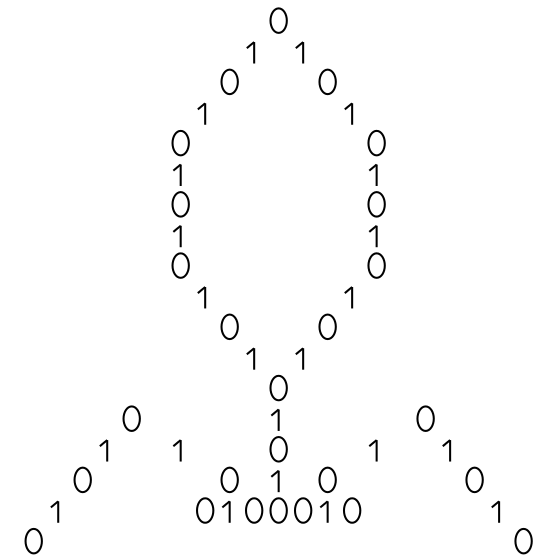
\includegraphics[width=90pt,height=90pt]{images/fudepan.png}\\
                \vfill
                \begin{scriptsize}
                    \textsc{FuDePAN} \\
                \end{scriptsize}
                \begin{tiny}
                    \textsc{Fundaci\'on para el Desarrollo de la Programaci\'on en \'Acidos Nucleicos} \\[1cm]    
                \end{tiny}
            \end{center}
        \end{minipage}

        \vspace{3cm}
        
        \textsc{\small{Trabajo Final}}\\
        \textsc{\footnotesize{Licenciatura en Ciencias de la Computaci\'on}}\\
        
        \HRule\\[0.1cm]
        \textbf{\Large{CombEng}\\[0.3cm]
                \large Implementation of a Distributed Combinatory Engine over FuD and its Application to Bioinformatic Problems}\\[0.1cm]
        \HRule\\[0.4cm]

        \vspace{3.5cm}

        \begin{normalsize}
            \center{\small{\textsc{Autores}}}\\
            \textbf{Bettiol}, Favio\\
            \textbf{Diaz}, Diego
        \end{normalsize}
            
        \vspace{.5cm}
        
        \begin{minipage}{0.4\textwidth}
            \begin{center}
                \center{\small{\textsc{Director}}} \\
                \large{\textbf{Biset}, Guillermo}
            \end{center}
        \end{minipage}
        \begin{minipage}{0.4\textwidth}
            \begin{flushright} 
            \center{\small{\textsc{Co-Director}}} \\
            \large{\textbf{Gutson}, Daniel}
            \end{flushright}
        \end{minipage}

        \vfill
        {\large 7 de diciembre de 2011}
    \end{center}

\end{titlepage}

\newpage
\thispagestyle{empty}
\mbox{}
\chapter*{Agradecimientos}
Este trabajo no se habr\'ia podido realizar sin la colaboraci\'on de muchas personas que nos han brindado su ayuda, sus conocimientos y su apoyo. Queremos agradecerles a todos ellos por cuanto han hecho por nosotros para que este trabajo saliera adelante de la mejor manera posible.

Queremos agradecerle especialmente a los dos directores de esta tesis: Daniel Gutson y Guillermo Biset. Ellos han sido los mentores de este proyecto y son quienes confiaron en nosotros para que lo llevemos adelante. Nos han guiado con mucha dedicaci\'on y paciencia durante el desarrollo del mismo, y, gracias a esto, hemos adquirido valiosos conocimientos, tanto en aspectos acad\'emicos como en muchos otros m\'as.

A los autores del proyecto \emph{RecAbs}, Emanuel Bringas y Mariano Bessone, por estar presentes siempre que necesitamos ayuda con su proyecto.
Esperamos haberles sido de tanta utilidad como ustedes lo han sido para nosotros.

Al autor del proyecto \emph{VAC-O}, Santigo Videla, y a los autores del proyecto \emph{ASO}, Andr\'es Peralta Godoy y Ezequiel Velez, quienes fueron
consultados varias veces por sus trabajos, de los cuales se hace un extenso uso de los mismos.

A Cecilia Cammisa y Daniel Rabinovich por ense\~narnos y corregirnos innumerables cosas en cuanto a Biolog\'ia. Cuando la situaci\'on lo requer\'ia, 
han ayudado con la mejor predisposici\'on.

A Marcelo Arroyo y Nazareno Aguirre por su buena voluntad para ayudarnos con las formalidades requeridas por la universidad que este trabajo
demand\'o.

Al Departamento de Computaci\'on y a su director, en su momento Nazareno, por facilitarnos las salas de m\'aquinas para realizar pruebas a escalas un
poco mayores.

A todos los miembros de la fundaci\'on \fudepan\ y, en especial, a su presidente Daniel Gutson, por ser personas que, sin esperar nada a cambio,
trabajan incansablemente s\'olo por su amor a la investigaci\'on.

Finalmente, y no por eso menos importante, sino todo lo contrario, queremos agradecerles muy especialmente a nuestras familias por habernos apoyado incondicionalmente a lo largo de toda la carrera. Esperamos que este trabajo, y el logro que el mismo conlleva, sea una m\'inima retribuci\'on a tantas cosas que ustedes nos han brindado durante los \'ultimos 6 a\~nos de estudio.

\newpage

\tableofcontents

\newpage

\listoffigures

\newpage

\listoftables


\newpage
\nocite{*} 


\thispagestyle{empty}
\mbox{}
\part{Preliminares}

\thispagestyle{empty}
\mbox{}
\chapter{Introducci\'on}
  Los virus tales como el HIV (Virus de Inmunodeficiencia Humana) no pueden reproducirse por s\'i mismos, sino que precisan de la maquinaria celular para lograrlo. Por esta raz\'on, deben infectar a las c\'elulas de un organismo vivo para duplicarse, es decir, hacer copias nuevas de ellos mismos. A menudo, el sistema inmunol\'ogico elimina las part\'iculas virales que pueden ingresar en un organismo, no obstante, el HIV ataca el sistema inmunol\'ogico mismo, aquel que se encarga de eliminarlas.

  Por otro lado, el SIDA (S\'indrome de Inmunodeficiencia Adquirida) es una afecci\'on m\'edica. A una persona infectada por el virus HIV
  se le diagnostica SIDA cuando su sistema inmunol\'ogico es demasiado d\'ebil para combatir las infecciones.

  Desde su primera manifestaci\'on, all\'a por el a\~no 1981, hasta la actualidad, el tratamiento de la infecci\'on por el HIV ha 
  sido, y seguir\'a siendo, foco de numerosas investigaciones. Se han propuesto diferentes enfoques a lo largo de estos a\~nos como terapias para tratamiento del SIDA, pero la terapia m\'as com\'unmente utilizada consiste en una combinaci\'on de diferentes antirretrovirales. 
  
  Desde 1987, a\~no en que se aprob\'o el uso de la \textit{zidovudine}\footnote{Inhibidor nucle\'osido de transcriptasa reversa. Se vende bajo los nombres de \textbf{Retrovir} y \textbf{Retrovis}.} en la prevenci\'on de la replicaci\'on del HIV, hasta 1995, la terapia consist\'ia en la administraci\'on de un solo antirretroviral para disminuir la carga viral en sangre, tratamiento m\'as conocido como monoterapia. En 1996, los avances significativos sobre el comportamiento del HIV y la expansi\'on en la s\'intesis de diferentes clases de antirretrovirales, hicieron posible el paso de la monoterapia hacia terapias combinatorias de alta eficacia, cuyo fin radica en la administraci\'on simult\'anea de distintos antirretrovirales pertenecientes a diferentes grupos. Esta terapia con ``cocktails'' de antirretrovirales que recibe el nombre de Tratamiento Antirretroviral de Gran Actividad o HAART (\emph{Highly Active Antiretroviral Therapy})\cite{haart} ha tenido un efecto dram\'atico dado que, en esencia, la terapia de combinaci\'on sofoca las mutantes de HIV antes de que tengan chances de florecer.

  Sin embargo, no todas las personas se adhieren del mismo modo al tratamiento antirretroviral. La adherencia es una cuesti\'on de vital
  importancia ya que contribuye a evitar la resistencia a los f\'armacos, de otra forma, se puede dar lugar a la aparici\'on de mutantes del HIV que
  ya no sean susceptibles a los efectos de la medicaci\'on que se toma.
  
  Ahora bien, \textit{?`El desarrollo de mutantes asociadas a la resistencia de los antirretrovirales, tiene alguna implicancia en la estructura 
  secundaria del ARN Viral?}

  Este trabajo intenta dar un abordaje inicial a lo antes mencionado, me\-dian\-te el desarrollo de una aplicaci\'on de 
  software que, tomando como entrada una secuencia inicial del virus y los antirretrovirales disponibles hasta el momento, permita analizar c\'omo 
  las diferentes terapias pueden afectar, o no, a la \textbf{estructura secundaria} y si esta posible afecci\'on puede ser un factor en la evoluci\'on viral.

  Para ello, se obtiene el valor $\Delta$G del virus original y se lo compara con aquellos $\Delta$G de las secuencias mutantes resultantes de 
  aplicar una terapia y con secuencias que, a pesar de tener la misma secuencia aminoac\'idica que las resistentes, no se presentan en los pacientes.

  Dado que todo este proceso es muy costoso computacionalmente, se opta por desarrollar la aplicaci\'on como una capa de un framework para
  aplicaciones distribuidas, desarrollado por integrantes de la fundaci\'on y que recibe por nombre \fud \ (\textbf{F}uDePAN \textbf{U}biquitous
  \textbf{D}istribution).

  Como parte de este trabajo final, se realiza el acoplamiento de otra nueva capa al framework proveyendo, entre otras cosas, un motor combinatorio.
  Este \'ultimo es qui\'en facilitar\'a la obtenci\'on de las posibles terapias.

  La decisi\'on de implementar esta \'ultima capa se debe a la gran cantidad de problemas que se presentan en la fundaci\'on, de caracter
  bioinform\'atico, que requieren de la generaci\'on de combinaciones en diferentes sabores y el problema tratado aqu\'i no escapa a ello.

\chapter{Marco Te\'orico}
  En este cap\'itulo se introducir\'a al lector en el framework \fud \ y en los conceptos b\'asicos de biolog\'ia para un mayor entendimiento de la
  aplicaci\'on implementada como parte de este trabajo final.

  \section{El Framework \fud}
    Computar grandes conjuntos de datos es una parte importante de las ciencias de la computaci\'on, mucha informaci\'on importante es inherentemente
    complicada de comprimir y, adem\'as, los recursos para procesar estos conjuntos de datos son usualmente costosos. Las organizaciones sin fines de
    lucro, las instituciones educativas y similares deben encontrar otros caminos para administrar sus requerimientos de procesamientos mientras
    mantienen sus costos lo m\'as bajo posible. Existen muchas herramientas para lograr una forma de computaci\'on distribuida en bajo costo.

    \fud \ (del acr\'onimo \textbf{F}uDePAN \textbf{u}biquitous \textbf{D}istribution) consiste en el dise\~no e implementaci\'on de un framework
    abstracto para implementar algoritmos distribuidos independientes de las herramientas antes mencionadas, de los sistemas de comunicaci\'on 
    subyacentes o alg\'un otro problema espec\'ifico.

    Este framework es un sistema separado en las capas de \textit{aplicaci\'on}, 
    \textit{administraci\'on} y \textit{distribuci\'on} combinando los conceptos de cliente-servidor y Divide \& Conquer. Tanto el cliente como el
    servidor se encuentran organizados en estos tres niveles (muy) separados, cada uno de ellos con una \'unica responsabilidad bien definida.
    \begin{figure}[H] \hspace{.60cm}
      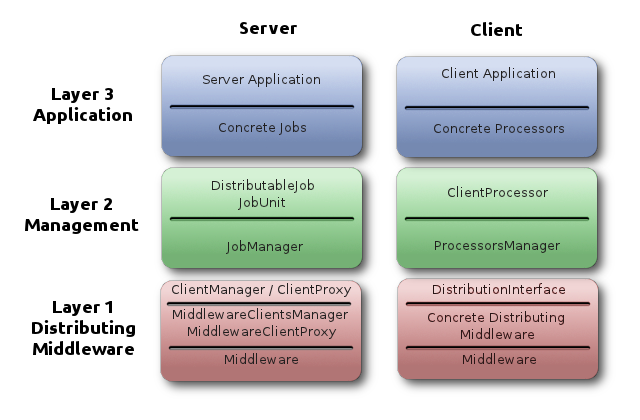
\includegraphics[scale=.51]{images/AbstractLayers.png}
      \caption{Vista abstracta de las capas en una instancia de uso de \fud} \label{disenioFud}
    \end{figure}
    La comunicaci\'on entre los diferentes niveles se encuentra estrictamente limitada, es decir, por cada nivel existe un \'unico punto de comunicaci\'on 
    ya sea para comunicarse con la capa superior o con la inferior siguiendo el enfoque OSI para redes.
    
    A continuaci\'on, muy brevemente, se explican cada una de las capas:
    \subsection{Application Layer (L3)}
    Este nivel provee los componentes que contienen todos los aspectos del dominio del problema. Estos aspectos incluyen todas las definiciones de los
    datos usados y su manipulaci\'on correspondiente, como as\'i tambi\'en todos los algoritmos relevantes para la soluci\'on al problema en general. Se debe
    tener en cuenta que bajo ninguna circunstancia esta capa pertenecer\'a a \fud \ pero su presencia es de ayuda para mostrar el uso del framework.

    \subsection{Job Management Layer (L2)}
    La responsabilidad de esta capa es manejar los trabajos que se desean distribuir como as\'i tambi\'en generar las unidades de trabajo que ser\'an
    entregadas a los clientes para su procesamiento. Estas unidades de trabajo llegan a su cliente correspondiente gracias a la capa m\'as baja, 
    encargada de la distribuci\'on. Una vez finalizado el procesamiento, es el nivel 2 quien informa que todo ha terminado y otorga los resultados a la capa superior.
  \newpage
    \subsection{Distributing Middleware Layer (L1)}
    A partir de esta vista abstracta del dise\~no, se debe notar que L1 solo constituye un esquema de administraci\'on de clientes en particular. Tal y
    como se observa en la figura \ref{disenioFud}, en ambos lados las partes fijas son las intarfaces del middleware, mientras que las
    implementaciones concretas son las partes variables (por ejemplo, BOINC o MPI).

    Notar que si se toma al proyecto \fud \ por separado, el mismo constituye una biblioteca que esta parcialmente implementada siempre y cuando el
    middleware de distribuci\'on est\'andar (boost::asio) sea removido. Esto lleva a que se pueden obtener diferentes sabores de la biblioteca \fud \
    con s\'olo reemplazar la capa de distribuci\'on (L1) por alguna otra. Por ejemplo, se podr\'ia utilizar MPI
    \footnote{\url{http://www.mcs.anl.gov/research/projects/mpi/}}, recomendado para clusters locales donde sus computadoras disponen de una 
    interconexi\'on veloz. Otra alternativa podr\'ia ser BOINC\footnote{\url{http://boinc.berkeley.edu/}} que posee una riqueza extrema en procesamiento,
    pero \'esta es llevada a cabo pagando el precio de la comunicaci\'on a trav\'es de Internet (la cual es bastante m\'as baja en velocidad con 
    respecto a otras configuraciones como Ethernet, infiniband, etc.). Estas diferentes implementaciones de la capa 1 deben ser intercambiables,
    es decir, uno puede variar entre ellas y el problema debe continuar siendo solucionable correctamente.

  \section{RNA Folding Free Energy}
  Como parte de esta tesis se implement\'o una aplicaci\'on de gran inter\'es para la fundaci\'on \fudepan \footnote{http://www.fudepan.org.ar/}. La descripci\'on
  e implementaci\'on de la misma se encuentra en el cap\'itulo \ref{RNAFFE_chapter}, en esta secci\'on presentamos los conceptos b\'asicos necesarios para comprender
  con mayor detalle la aplicaci\'on.

  \subsection{Organismos, Mol\'eculas y C\'elulas}
  \subsubsection{Organismos}
  Conjunto de biomol\'eculas org\'anicas e inorg\'anicas organizadas de manera especifica para cumplir determinadas funciones e interactuar con el medio en que se encuentran.
  
  \subsubsection{Mol\'eculas  Org\'anicas}
  Hay dos tipos de mol\'eculas org\'anicas b\'asicas:

  \begin{itemize}
    \item \emph{Nucle\'otidos}:
      Peque\~nas mol\'eculas constituyentes de macromol\'eculas de mayor complejidad. Los 5 tipos de nucle\'otidos m\'as importantes son:
      \begin{enumerate}
        \item Adenina (A) compone el ADN y el ARN.
        \item Guanina (G) compone el ADN y el ARN.
        \item Timina (T) compone el ADN.
        \item Citosina (C) compone el ADN y el ARN.
        \item Uracilo (U) compone el ARN.
      \end{enumerate}


    \item \emph{Amino\'acidos}:
      Son mol\'eculas que conforman las prote\'inas y son esenciales para la vida. A continuaci\'on se muestra una tabla conteniendo todos los amino\'acidos 
      y sus abreviaciones.
      \begin{center}
        \begin{tabular}{|ccc|}
          \hline Nombre & Ab. 3 letras & Ab. 1 Letra \\ 
          \hline Alanine & Ala & A \\ 
          \hline Arginine & Arg & R \\ 
          \hline Asparagine & Asn & N \\ 
          \hline Aspartic acid & Asp & D \\ 
          \hline Cytesine & Cys & C \\ 
          \hline Glutamic acid & Glu & E \\ 
          \hline Glutamine & Gln & Q \\ 
          \hline Glycine & Gly & G \\ 
          \hline Histidine & His & H \\ 
          \hline Isoleucine & Ile & I \\ 	
          \hline Leucine & Leu & L \\ 
          \hline Lysine & Lys & K \\ 
          \hline Methionine & Met & M \\ 
          \hline Phenylalanine & Phe & F \\ 
          \hline Proline & Pro & P \\ 
          \hline Serine & Ser & S \\ 
          \hline Threonine & Thr & T \\ 
          \hline Tryptophan & Trp & W \\ 
          \hline Tyrosine & Tyr & Y \\ 
          \hline Valine & Val & V \\ 
          \hline 
        \end{tabular} 
      \end{center}
  \end{itemize}


  \subsubsection{Macromol\'eculas}
  Son estructuras biol\'ogicas conformadas por un determinado n\'umero de mol\'eculas org\'anicas. Hay cuatro tipos de macromol\'eculas, \'Acidos Nucleicos, Prote\'inas, 
  Gl\'ucidos y L\'ipidos. S\'olo explicaremos las primeras dos ya que son las \'unicas relevantes para la aplicaci\'on:
  \begin{itemize}
    \item \emph{\'Acidos Nucleicos}: Est\'an conformados por secuencias de nucle\'otidos espec\'ificas, que son utilizadas por todos los organismos para almacenar su informaci\'on gen\'etica. La misma, est\'a codificada mediante sucesivos codones, los cuales est\'an conformados por tripletes de nucle\'otidos que codifican un amino\'acido. Dos de los \'acidos nucleicos m\'as importantes son:
      \begin{enumerate}
        \item \textbf{ADN (\'Acido Desoxirribonucleico)}: Contiene la informaci\'on gen\'etica para el desarrollo y el funcionamiento de los organismos vivos
	  y de algunos virus, la cual se hereda de generaci\'on en generaci\'on. Est\'a formado por una doble cadena de nucle\'otidos, en la que las dos hebras est\'an unidas a trav\'es de las bases complementarias, seg\'un el modelo propuesto por Watson y Crick en 1953.
        \item \textbf{ARN (\'Acido Ribonucleico)}: Consiste en una hebra de cadena simple, la cual usualmente es trascripta a partir de una porci\'on de ADN y se utiliza posteriormente en la c\'elula para la s\'intesis de prote\'inas. Algunos virus poseen ARN como \'unico material gen\'etico cuya monohebra puede plegarse, dando lugar a lo que se conoce como estructura secundaria, la cual se analizar\'a m\'as adelante.
      \end{enumerate}

    \item \emph{Prote\'inas:}
      Est\'an formadas por secuencias de amino\'acidos espec\'ificas, que adoptan una conformaci\'on tridimensional determinada debido a las interacciones electrost\'aticas existentes entre los residuos de sus amino\'acidos constituyentes. Este arreglo tridimensional la habilita para realizar una funci\'on en particular.
  \end{itemize}

  %\begin{figure}[h!]
  %\centering
  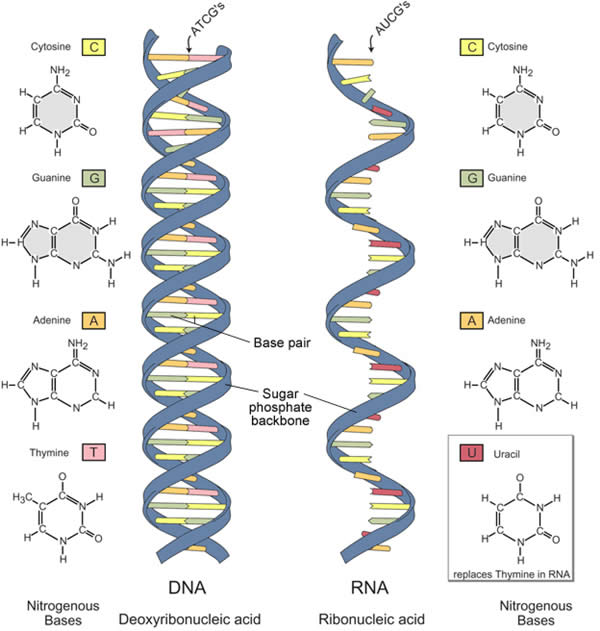
\includegraphics[width=\linewidth]{images/dna_rna.png}
  %\caption{C\'elulas Procariota y Eucariota.} 
  %\end{figure} 

  \subsubsection{C\'elulas}
  Son unidades b\'asicas que conforman el organismo y dentro de \'estas ocurren todas las funciones vitales. Adem\'as contienen la informaci\'on gen\'etica en su ADN, la cual se transmite a las c\'elulas hijas. Existen dos tipos:
  \begin{enumerate}
    \item \textit{Procariotas}: Carecen de membrana nuclear.
    \item \textit{Eucariotas}: Poseen un n\'ucleo bien definido mediante una membrana nuclear que contiene al ADN.
  \end{enumerate}

  \subsection{La Estructura Secundaria Del ARN}\label{estructuraSecundariaARN}
  El plegamiento de una secuencia de ARN entre sus bases complementarias determina lo que se denomina \emph{estructura secundaria de ARN}. Conocer la 
  estructura secundaria es fundamental para comprender el funcionamiento de los distintos tipos de ARN y de la c\'elula en general. Existen diferentes
  tipos de ARN, distingui\'endose entre ellos:
  \begin{itemize}
    \item \textit{Messenger ARN} (mRNA).
    \item \textit{Ribosomal ARN} (rRNA).
    \item \textit{Transfer ARN} (tRNA).
  \end{itemize}

  La existencia del t\'ermino \emph{estructura secundaria} nos hace suponer tambi\'en la existencia de una \emph{estructura primaria}. Como se mencion\'o, dicha estructura queda representada mediante una secuencia de nucle\'otidos. Tambi\'en existe la estructura terciaria de ARN, pero se la deja a un lado por no
  ser relevante en este trabajo.

  \begin{definition}
    \label{rna_primary}
    La estructura primaria del ARN, es una secuencia de nucle\'otidos de longitud
    $n$, $A=a_{1}a_{2}a_{3}\dots a_{n}$ con $a_{i} \in \left\lbrace A, U, G, C
    \right\rbrace$ 
  \end{definition}

  \begin{definition}
    \label{rna_secondary}
    Dada una estructura primaria o secuencia de RNA de longitud $n$, la
    estructura secundaria es un conjunto S de pares $(i,j)$ con $1\leq i < j \leq
    n$ tal que para todo, $(i,j), (i',j') \in S$ se satisfacen las tres siguientes
    condiciones:
    \begin{itemize}
      \item $j-i > 3$
      \item $i=i' \Leftrightarrow j=j'$
      \item $i< i'\Rightarrow i < i' < j' < j \lor i < j < i' < j'$ 
    \end{itemize}
  \end{definition}

  \subsection{Energ\'ia Libre y Estabilidad}
  El concepto de ``Energ\'ia Libre'' hace referencia a la energ\'ia total contenida en un sistema, como por ejemplo una mol\'ecula de ARN con una estructura secundaria, la cual le permite al mismo realizar trabajo. Una mol\'ecula de ARN puede estar dotada de una cierta cantidad de energ\'ia libre mediante interacciones el\'ectricas no neutralizadas en su estructura primaria, por lo tanto, esta energ\'ia se utilizar\'a para plegar la misma hacia una estructura secundaria m\'as estable. De este modo, un ARN con una estructura secundaria estable, implica una mol\'ecula en la cual sus interacciones el\'ectricas entre nucle\'otidos se hallan completamente neutralizadas. Se podr\'ia inferir que si una secuencia viral de ARN mutada tiene energ\'ia libre m\'inima, la misma no variar\'a su estructura secundaria por s\'i sola. 
  
  \subsection{Virus HIV}
  Los virus son entidades infecciosas microsc\'opicas que pueden multiplicarse dentro de las c\'elulas de un organismo dado. El virus HIV (\emph{Human immunodeficiency virus}) infecta a c\'elulas vitales del sistema inmunol\'ogico humano, tales como los \textit{Linfocitos T} (espec\'ificamente los que contienen receptores CD4$^+$), los \textit{macr\'ofagos} y las \textit{c\'elulas dendr\'iticas}. Las CD4$^+$ son un sub-grupo de los linfocitos, un tipo de gl\'obulos
  blancos, los cuales desempe\~nan un rol importante en el establecimiento y maximizaci\'on del sistema de defensa de un organismo.

  La infecci\'on con HIV lleva a un nivel bajo de c\'elulas T CD4$^+$. En el instante en que \'estas llegan a un nivel cr\'itico, se pierde la
  inmunidad celular y el organismo, progresivamente, se vuelve cada vez m\'as susceptible a otras infecciones oportunistas.

  \subsection{SIDA}
  El SIDA, del acr\'onimo \textbf{S}\'indrome de \textbf{I}nmunodeficiencia \textbf{A}dquirida, es una enfermedad que afecta a los humanos infectados
  por el HIV tipo 1. Se dice que una persona padece de SIDA cuando su organismo, debido a la inmunodeficiencia provocada por el HIV, no es capaz de ofrecer
  una respuesta inmune adecuada contra las infecciones.

  Cabe destacar la diferencia entre estar infectado por el HIV y padecer de SIDA. Una persona infectada por el HIV es \textit{seropositiva}\footnote{el
  t\'ermino seropositivo se aplica a una condici\'on inmunitaria, caracterizada por la presencia de un anticuerpo espec\'ifico en sangre, creado frente
  a un ant\'igeno que puede provenir de un agente infeccioso como de uno no infeccioso.} la cual luego desarrolla un cuadro de SIDA cuando su nivel de
  linfocitos T CD4$^+$ desciende por debajo de 200 c\'elulas por mililitro de sangre.

  \subsection{Antirretrovirales}
  Los f\'armacos utilizados en tratamientos actuales para combatir las infecciones con HIV son denominados antirretrovirales. Existe una variedad de estos
  provenientes de distintos laboratorios, cada uno con sus respectivas caracter\'isticas, los cuales se clasifican por su rango de acci\'on en dos clases: los \emph{Protease Inhibitors} (PI) y \emph{Reverse Transcriptase Inhibitors}. Dentro de la segunda clase hay dos sub-tipos que son los \emph{Nucleotide Reverse Transcriptase Inhibitors} (NRTI) y los \emph{Non-Nucleotide Reverse Transcriptase Inhibitors} (NNRTI). Existen otras dos clases m\'as recientes que son los \emph{Fusion or Entry Inhibitors} y los \emph{Integrase Inhibitors}. El objetivo de aplicar antirretrovirales a los pacientes es inhibir la replicaci\'on del virus por un tiempo indeterminado.

  A continuaci\'on se muestra una tabla conteniendo los antirretrovirales aprobados por la FDA (Food and Drugs Administration
  \url{http://www.fda.gov/MedicalDevices/default.htm}).


  M\'ultiples Clases Combinadas (Multi-class combinations):
  \begin{center}
    \begin{tabular}{|c|c|c|}
      \hline Combinaci\'on & Comercial & Aprobaci\'on \\ 
      \hline EFV + TDF + FTC & Atripia & 12-Jul-06 \\ 
      \hline d4T + 3TC + NVP & - & Tentative only* \\ 
      \hline AZT + 3TC+ NVP & - & Tentative only* \\ 
      \hline 
    \end{tabular}
  \end{center}

  Inhibidores de Transcriptasa Reversa Nucle\'osidos (NRTIs):

  \begin{center}
    \begin{tabular}{|c|c|c|c|}
      \hline Abreviaci\'on & Gen\'erico & Comercial & Aprobaci\'on \\ 
      \hline 3TC & lamivudine & Epivir & 17-Nov-95 \\ 
      \hline ABC & abacavir   & Ziagen & 17-Dec-98  \\ 
      \hline AZT o ZDV & zidovudine & Retrovir & 19-Mar-87 \\ 
      \hline d4T & stavudine & Zerit & 24-Jun-94  \\ 
      \hline ddI & didanosine & Videx EC & 31-Oct-00  \\ 
      \hline FTC & emtricitabine & Emtriva & 02-Jul-03 \\ 
      \hline TDF & tenofovir & Viread & 26-Oct-01  \\ 
      \hline 
    \end{tabular}
  \end{center}

  Inhibidores de Transcriptasa Reversa No Nucle\'osidos (NNRTIs):

  \begin{center}
    \begin{tabular}{|c|c|c|c|}
      \hline Abreviaci\'on & Gen\'erico & Comercial & Aprobaci\'on \\ 
      \hline DLV & delavirdine & - & 04-Apr-97 \\ 
      \hline EFV & efavirenz   & Sustiva & 17-Sep-98 \\ 
      \hline ETR & etravirine & Intelence & 18-Jan-08 \\ 
      \hline NVP & nevirapine & Viramune & 21-Jun-96 \\ 
      \hline 
    \end{tabular}
  \end{center}

  NRTIs Combinados (Combined NRTIs):

  \begin{center}
    \begin{tabular}{|c|c|c|}
      \hline Combinaci\'on & Comercial & Aprobaci\'on \\ 
      \hline ABC + 3TC & Epzicom (US) & 02-Aug-04  \\ 
      \hline ABC + AZT + 3TC & Trizivir & 14-Nov-00 \\ 
      \hline AZT + 3TC & Combivir & 27-Sep-97  \\ 
      \hline TDF + FTC & Truvada & 02-Aug-04  \\ 
      \hline d4T + 3TC & - & Tentative only*  \\ 
      \hline 
    \end{tabular}
  \end{center}

  Inhibidores de Proteasa (Protease Inhibitors) (PIs):

  \begin{center}
    \begin{tabular}{|c|c|c|c|}
      \hline Abreviaci\'on & Gen\'erico & Comercial & Aprobaci\'on \\
      \hline APV & amprenavir & Agenerase & 15-Apr-99  \\ 
      \hline FOS-APV & fosamprenavir & Lexiva (US) & 20-Oct-03 \\ 
      \hline ATV & atazanavir & Reyataz & 20-Jun-03 \\ 
      \hline DRV & darunavir & Prezista & 23-Jun-06 \\ 
      \hline IDV & indinavir & Crixivan & 13-Mar-96 \\ 
      \hline LPV/RTV & lopinavir + ritonavir & Kaletra & 15-Sep-00 \\ 
      \hline NFV & nelfinavir & Viracept & 14-Mar-97	 \\ 
      \hline RTV & ritonavir & Norvir & 01-Mar-96 \\ 
      \hline SQV & saquinavir & Invirase & 06-Dec-95 \\ 
      \hline TPV & tipranavir & Aptivus & 22-Jun-05 \\ 
      \hline 
    \end{tabular} 
  \end{center}

  Inhibidores de Fusi\'on o Entrada (Fusion or Entry Inhibitors):

  \begin{center}
    \begin{tabular}{|c|c|c|c|}
      \hline Abreviaci\'on & Gen\'erico & Comercial & Aprobaci\'on \\ 
      \hline T-20	& enfuvirtide &	Fuzeon & 13-Mar-03  \\ 
      \hline MVC & maraviroc &Celsentri & 18-Sep-07 \\ 
      \hline 
    \end{tabular}
  \end{center}

  Inhibidores de Integrasa (Integrase Inhibitors):

  \begin{center}
    \begin{tabular}{|c|c|c|c|}
      \hline Abreviacia\'on & Gen\'erico & Comercial & Aprobaci\'on \\ 
      \hline RAL & raltegravir & Isentress & 12-Oct-07  \\ 
      \hline 
    \end{tabular} 
  \end{center}

  \subsection{Fracaso, o Fallo, Terap\'eutico Para El HIV}\label{fracasoTerapeutico}
  El fracaso terap\'eutico, o de tratamiento, ocurre cuando los medicamentos para HIV no pueden controlar la infecci\'on de un modo eficiente.
  Existen tres tipos de fracaso terap\'eutico: \textbf{fallo virol\'ogico}, \textbf{fallo inmunol\'ogico} y \textbf{fallo cl\'inico}.

  El fracaso virol\'ogico ocurre cuando los antirretrovirales no pueden disminuir la carga viral en sangre. De este modo, aunque el paciente est\'e tomando los 
  medicamentos proscritos, la cantidad de virus en sangre no disminuye o bien se eleva repetidamente.

  El fracaso inmunol\'ogico ocurre cuando el sistema inmunitario no responde a los medicamentos antirretrovirales. De este modo, aunque tome los medicamentos, el recuento de linfocitos CD4+ no disminuye ni se incrementa.

  El fracaso cl\'inico se presenta cuando, a pesar que el paciente toma los medicamentos antirretrovirales, persisten los s\'intomas de infecci\'on por VIH.

  Los tres tipos de fracaso terap\'eutico pueden ocurrir solos o simult\'aneamente. Por lo general, primero ocurre el fracaso virol\'ogico, seguido por el
  fracaso inmunol\'ogico y luego se presenta el fracaso cl\'inico. Pueden ocurrir en un lapso de meses o a\~nos entre s\'i mismos.

  \subsubsection{?`Cu\'ales son los factores de riesgo para el fracaso terap\'eutico?}
  Los factores que pueden incrementar el riesgo del fracaso terap\'eutico incluyen:
  \begin{itemize}
    \item Fracaso terap\'eutico previo
    \item \textbf{Resistencia farmacol\'ogica} (o resistencia al medicamento)
    \item Falta de adherencia al tratamiento
    \item El organismo no absorbe debidamente los medicamentos antirretrovirales
    \item Cualquier otra enfermedad o afecci\'on
    \item Mala salud antes de comenzar el tratamiento
    \item Efectos secundarios de los medicamentos o interacciones con otros medicamentos
    \item Abuso de sustancias t\'oxicas que ocasionan falta de adherencia al tratamiento.
  \end{itemize}

  \subsection{Otros T\'erminos}
  \begin{description}
    \item \textbf{Adherencia al tratamiento:} consiste en seguir (acatar) cuidadosamente un r\'egimen de tratamiento. Eso incluye tomar la dosis correcta
      de un medicamento en el momento adecuado, exactamente como se lo recetaron.
    \item \textbf{Carga viral:} cantidad de HIV en una muestra de sangre. La carga viral mide qu\'e tan bien est\'an controlando la infecci\'on los
          antirretrovirales.
    \item \textbf{Pruebas de resistencia farmacol\'ogica:} pruebas de laboratorio para determinar si el VIH de una persona es resistente a cualquier
          medicamento antirretroviral.
    \item \textbf{Recuento de linfocitos CD4+:} Un recuento CD4+ es la cantidad de linfocitos CD4+ en una muestra de sangre. El recuento CD4+ mide la salud
      del sistema inmunitario.
    \item \textbf{Resistencia farmacol\'ogica:} El HIV puede mutar (EL ARN cambia su secuencia de nucle\'otidos para hacerse resistente a un antirretroviral). El VIH alterado se puede multiplicar incluso en presencia de medicamentos antirretrovirales que normalmente matar\'ian el virus. Uno o m\'as medicamentos en un r\'egimen de tratamiento pueden volverse ineficaces como resultado de la resistencia farmacol\'ogica.
    \item \textbf{Resistencia inmunol\'ogica:} Las nuevas pruebas no muestran aumento del recuento de linfocitos CD4+ a pesar del tratamiento. Un descenso en
      el recuento CD4+ mientras el paciente toma antirretrovirales puede indicar tambi\'en fracaso inmunol\'ogico.
  \end{description}


\chapter{Metodolog\'ia de Trabajo}
%(completar testing y analisis estatico de cod)}

\section{Pr\'acticas De Software}

\begin{itemize}
 \item \textbf{Dise\~no:} Durante el desarrollo de \combeng, aproximadamente el 50 por ciento del tiempo fue dedicado al dise\~no. En este porcentaje esta 
   incluido el dise\~no original y algunos cambios que debieron ser hechos durante la implementaci\'on. 
   Para obtener como resultado un dise\~no que respeta, entre otras cosas, dos principios b\'asicos: Simplicidad y ocultamiento de la informaci\'on, 
   se utilizaron Patrones de Dise\~no\cite{Gamma95} y UML.
 \item \textbf{Construcci\'on de c\'odigo:} Aproximadamente el 30 por ciento del tiempo fue dedicado a la construcci\'on del c\'odigo. Cada vez que se implemento un nuevo componente se cheque\'o la integraci\'on del mismo con todo el proyecto. Cuando superaba la prueba, el c\'odigo era subido al \textbf{trunk} del repositorio.
 \item \textbf{Revisiones:} La mayor\'ia de las operaciones \emph{commits} realizadas (incluyendo c\'odigo, diagramas, documentos de responsabilidades, etc.) fueron revisadas por al menos dos personas. No solo se resaltaron errores, sino tambi\'en cuestiones en cuando a calidad y eficiencia. Cada vez que se encontr\'o un error o sugerencia, una nueva revisi\'on fue creada conteniendo la soluci\'on.
 \item \textbf{Seguimiento de issues:} Los Bugs y defectos del proyecto fueron reportados como Issues. Luego, para cada issue, se creo una nueva revisi\'on conteniendo la soluci\'on.
 \end{itemize}

\section{Gesti\'on de la Configuraci\'on}
Para desarrollar \combeng \ y algunas aplicaciones de ejemplo (\textit{Clothes-Changer}, \textit{RNAFoldingFE}) fue necesario utilizar un manejador de versiones.
Para ello se manipul\'o un repositorio SVN alojado en GoogleCode con el fin de poder seguir la pista a todos los archivos que componen el proyecto.
Para m\'as informaci\'on acerca de qu\'e es y c\'omo utilizar Subversion puede consultarse los libros de O'Reilly [Sussman et al., 2008]. 

\section{GNU/Linux y Software Libre}
Tanto el sistema operativo como todas las herramientas que se usaron para el desarrollo del proyecto son libres. Hasta el momento, la licencia libre mas usada es GPL (General Public Licence), una copia de la misma pude ser encontrada en: \begin{verbatim} http://www.gnu.org/licenses/gpl-3.0.txt \end{verbatim}
\section{Herramientas}
Durante la realizaci\'on del proyecto fueron utilizadas distintas herramientas, todas ellas bajo licencia GPL. A continuaci\'on se muestra una lista 
de las m\'as usadas.

\subsection{GNU Toolchain}
Este proyecto fue realizado bajo el sistema operativo GNU/Linux, \'este cuenta con una serie de herramientas de gran utilidad e importancia. Las m\'as
utilizadas durante el desarrollo fueron:
\begin{itemize}
  \item \textbf{GCC (GNU Compiler Collection)}: Es un conjunto de compiladores creados por el proyecto GNU. GCC es software libre y se distribuye bajo
    licencia GPL. Estos compiladores se consideran est\'andar para sistemas operativos derivados de GNU.\footnote{\url{http://gcc.gnu.org/}}
  \item \textbf{GDB (GNU Debugger)}: Es un depurador portable que se puede utilizar en varias plataformas Unix y funciona para varios lenguajes de
    programaci\'on como C y C++ entre otros. GDB fue escrito por Richard Stallman en 1988, es software libre y se distribuye bajo licencia GPL.
    \footnote{\url{www.gnu.org/software/gdb/}}
  \item \textbf{CMake}: Es una familia de herramientas dise\~nadas para construir, probar y empaquetar software. CMake se utiliza para controlar el
    proceso de compilaci\'on del software usando archivos de configuraci\'on sencillos e independientes de la plataforma.\footnote{\url{www.cmake.org}}
 \end{itemize}

\subsection{Latex}
Todo este documento fue escrito en \LaTeX. Leslie Lamport en 1984, con la intenci\'on de facilitar el uso de \TeX \ (lenguaje de composici\'on tipográfica,
creado por Donald Knuth), cre\'o un sistema de composici\'on de textos. El mismo est\'a orientado especialmente a la creaci\'on de libros, documentos
cient\'ificos y t\'ecnicos que contengan f\'ormulas matem\'aticas. A dicho sistema lo llam\'o \LaTeX \ y est\'a formado por un gran conjunto de macros de
\TeX.

\subsection{Edici\'on}
\begin{itemize}
  \item \textbf{Gedit}: Editor de texto plano.\footnote{\url{http://projects.gnome.org/gedit/}}
  \item \textbf{Kile}: Editor para \LaTeX.\footnote{\url{http://kile.sourceforge.net/}}
 \item \textbf{vim+latexSuite}: Vim es un editor de texto altamente configurable construido para permitir la edici\'on de texto eficientemente.
     Se trata de una versi\'on mejorada del editor \textit{Vi} distribuido en la mayor\'ia de los sistemas UNIX. Adem\'as, latexSuite es un plugin para Vim,
     que integra una suite de \LaTeX.
\end{itemize}

\subsection{Gr\'aficos}
\begin{itemize}
  \item \textbf{Gimp}: Editor de im\'agenes.\footnote{\url{www.gimp.org}}
  \item \textbf{Bouml}: Editor de diagramas UML.\footnote{\url{http://bouml.free.fr/}}
  \item \textbf{UMLet}: Editor de diagramas UML.\footnote{\url{www.umlet.com}}
  \item \textbf{Dia}: Editor de diagramas de prop\'osito general.\footnote{\url{http://live.gnome.org/Dia}}
\end{itemize}

\subsection{Documentaci\'on}
\begin{itemize}
  \item \textbf{Doxygen}: Generador de documentaci\'on para m\'ultiples lenguajes.\footnote{\url{www.doxygen.org}}
\end{itemize}

\subsection{An\'alisis Est\'atico de C\'odigo}
\begin{itemize}
 \item gcc con flags
 \item cppcheck
\end{itemize}

\subsection{An\'alisis Estad\'istico}
\begin{itemize}
  \item \textbf{R}: Lenguaje y entorno de programaci\'on para realizar an\'alisis estad\'isticos y gr\'aficos.\footnote{\url{www.r-project.org}}.
\end{itemize}


\part{El Motor Combinatorio}

\thispagestyle{empty}
\mbox{}
\chapter{Combinatory Engine}
    \section{Descripci\'on del Problema}\label{descripcionproblema}
        El desarrollo del motor combinatorio, a partir de este momento ser\'a denominado \combeng, se vio originado por la necesidad de \fudepan \
        (Fundaci\'on para el Desarrollo de la Programaci\'on en \'Acidos Nucleicos) de contar con uno. En dicha fundaci\'on se presentan de ma\-ne\-ra
        recurrente, problemas de car\'acter bioinform\'atico. Una familia de ellos se ve caracterizada por compartir una o m\'as de las siguientes
        caracter\'isticas:
        \begin{itemize}
            \item Requerir un motor combinatorio para la generaci\'on de \'arboles de combinaciones.
            \item Utilizar mecanismos de poda sobre dichos \'arboles.
            \item Requerir un sistema de puntuaci\'on por cada una de las combinaciones (\textit{ranking} o \textit{scoring}).
        \end{itemize}

		El principal objetivo de este proyecto fue el de acoplar a \fud \ una capa que permita, a usuarios sin altos conocimientos en programaci\'on, 
		implementar soluciones a los problemas antes mencionados.

		La elecci\'on de acoplar \combeng \ como una nueva capa del framework \fud \ en lugar de crear un proyecto aparte, se debi\'o a que la mayor\'ia de los 
    problemas antes mencionados requieren un elevado nivel de c\'omputo, muchas veces ``\textit{imposible}'' de realizar en una \'unica computadora.

  \newpage
	\section{Nuevas Capas De FuD}
		A continuaci\'on, puede observarse un nuevo diagrama, al estilo OSI de redes, reemplazando al diagrama inicial del framework \fud \ 
		mostrando las diferentes capas:
    \begin{figure}[H] \hspace{.30cm}
        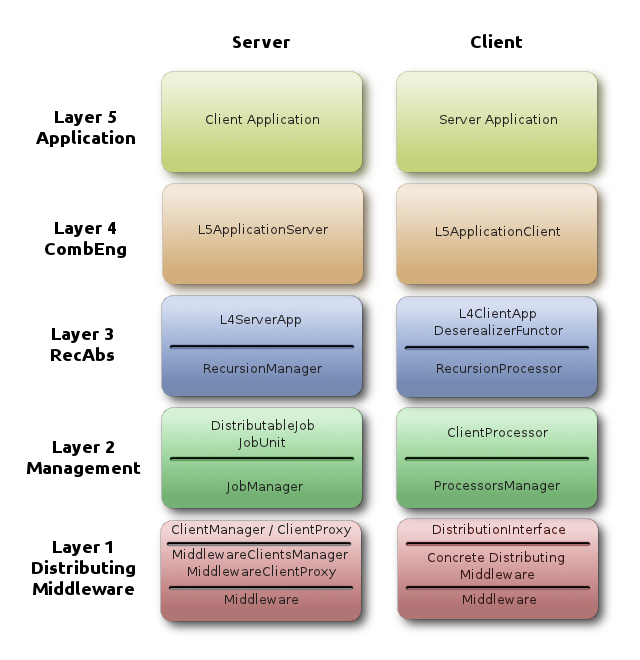
\includegraphics[scale=.51]{images/AbstractLayersRedesigned.png}
	         \caption{Vista abstracta de las nuevas capas en una instancia de uso de \fud}
	         \label{redisenioFud}
    \end{figure}
		
    Claramente se puede observar la existencia de otra nueva capa, denominada \recabs
    \footnote{\url{http://code.google.com/p/fud/source/browse/branches/FuD-duplex/layers/layer3-recabs/}}. La misma constituye otro proyecto de la
    fundaci\'on y es con el que \combeng \ interact\'ua, por lo que a continuaci\'on se explica en qu\'e consiste el mismo.
		
		\section{RecAbs}
			\recabs, al igual que el presente trabajo, surge como una propuesta de \fudepan. En tal fundaci\'on se necesitaba una biblioteca que facilitara
      la soluci\'on a un gran n\'umero de proyectos bioinform\'aticos, los cuales usan a la recursi\'on como mecanismo fundamental y poseen muchos
      factores de implementaci\'on en com\'un.

      La meta de este proyecto es identificar una abstracci\'on gen\'erica con una estructura com\'un a todas las soluciones recursivas a estos
      problemas de inter\'es y, al mismo tiempo, proveer una soluci\'on algor\'itmicamente eficiente para dichos proyectos. Esta abstracci\'on abarca
      la familia de problemas que cumplen las siguientes condiciones:

      \begin{itemize}
        \item la soluci\'on se adapte a un modelo recursivo. No obstante, se ajusta principalmente a aquellos problemas con definici\'on 
          inherentemente recursiva; y 
        \item los nodos del \'arbol de recursi\'on de la soluci\'on sean (horizontalmente) independientes.
      \end{itemize}

      Cabe destacar que, cualquiera sea el problema que se desee resolver por medio de \recabs, debe adoptar la forma recursiva, donde el paso
      inductivo conduce a problemas cada vez mas peque\~nos que, necesariamente, terminar\'an en, por lo menos, un caso base. Tambi\'en es
      significativo el segundo punto, el cual expresa que s\'olo se pueden solucionar problemas con la recursividad m\'as simple, es decir, 
      una vez llegado a las hojas esa ejecuci\'on se da por terminada y se informa un resultado, es imposible volver a pasos anteriores buscando
      diferentes caminos, como si lo permiten algoritmos de backtracking, combinatorios, etc.
			
			\subsection{Arquitectura}
				Dado que \recabs \ tambi\'en forma parte del framework, presenta el modelo cliente-servidor. El Servidor tiene la responsabilidad de iniciar 
				el proceso recursivo, administrar los pasos de recursi\'on que realizan los clientes y llevar el control de los resultados, mientras que el 
        cliente es el encargado de la resoluci\'on de un \textit{functor recursivo} (ver \ref{recursiveFunctor}). Durante la tarea de resoluci\'on, 
        el cliente puede pedir ayuda y solicitar el env\'io tanto de functores intermedios como de resultados al servidor.
				
				\recabs \ es un proyecto bastante extenso, por lo que s\'olo se har\'a menci\'on a aquellos componentes que interact\'uan de manera directa con 
				\combeng, es decir, aquellas interfaces de L3 que poseen servicios o funcionalidades a ser implementadas por capas superiores.
				
        \subsubsection{Lado Servidor}
					\begin{description}
            \item \textit{RecursionManager}: Es el ``handler'' del lado servidor. Cada paquete que sale de un cliente y llega a este \textit{manager},
              puede ser alguno de los siguientes tipos de paquetes:
              \begin{itemize}
                \item un \textbf{resultado}, parcial y relativo a la unidad de trabajo que se proces\'o, el cual es tratado de la manera que el usuario
                  desee. Indica, en el cliente, que se ha llegado a una hoja en el \'arbol de recursi\'on.
                \item un \textbf{mensaje intermedio} es cualquier dato transmitido de cliente a servidor sin llegar a una hoja o estado final en el
                  \'arbol, y por lo tanto no es un resultado. Tambi\'en es enviado (en cliente) y tratado (en servidor) como el usuario disponga.
                \item una \textbf{unidad de trabajo} a distribuir, la cu\'al ser\'a enviada a un cliente ocioso. Un \textit{trabajo} arribado es una
                  partici\'on del trabajo del cliente que lo envi\'o. 
              \end{itemize}
              Otro rol fundamental que juega el \textit{manager} es la de iniciar el proyecto implementado sobre \recabs. Para ello, el mismo cuenta
              con la ayuda de \textit{L4ServerApp} que nos brinda el functor inicial, el cual es apilado para distribuirlo al primer cliente ocioso
              que se encuentre, donde as\'i la iniciaci\'on del proceso recursivo.
						\item \textit{L4ServerApp}: La implementaci\'on de esta interfaz consta de los siguientes puntos:
              \begin{itemize}
                \item brindar el \textit{functor} inicial,
                \item definir qu\'e har\'a con los resultados a medida que lleguen, y
                \item definir el tratamiento de los mensajes intermedios (si es que los hubiera).
              \end{itemize}
              De estos requisitos, el primero es obligatorio mientras que los otros dos restantes son opcionales en la medida que la aplicaci\'on
              arroje resultados y mensajes intermedios.
					\end{description}

          \subsubsection{Lado Cliente}
					\begin{description}
						\item \textit{RecursiveProcessor}: Es el encargado de realizar la ejecuci\'on total (o parcial) del functor que fue asignado a un cliente.
						\item \textit{DeserializerFunctor}:	Provee los servicios de transformaci\'on de un paquete serializado a un functor recursivo.
            \item \textit{DistributionPolicy}: Es una interfaz que ofrece varios ``sabores'' de distribuci\'on ya implementados, as\'i como la posibilidad de
              extender este conjunto de pol\'iticas si el desarrollador quisiese. Cada pol\'itica establece cu\'ando un cliente debe distribuir o
              cu\'ando debe parar y, en caso positivo, cu\'anto debe distribuir. Cuando se menciona \textit{distribuir}, se hace referencia al env\'io 
              de unidades de trabajo a clientes ociosos que el server dispone.
					\end{description}

          \subsubsection{Com\'un a Ambos Lados}
					\begin{description}
            \item \textit{RecursiveFunctor}\label{recursiveFunctor}: es una abstracci\'on a la \textit{funci\'on recursiva} de una aplicaci\'on \recabs.
              Una aplicaci\'on deber\'a implementar la interfaz definida por \texttt{RecursiveFunctor}, este nuevo \textit{functor} (por ejemplo, 
              \texttt{ConcreteFunctor}) representar\'a la funci\'on que el usuario desee distribuir. Estos nuevos functores encapsulan la informaci\'on 
              espec\'ifica de cada aplicaci\'on, la cual es necesaria y suficiente para ser procesada por los clientes.
						\item \textit{SerializableRecursiveFunctor}: Es un RecursiveFunctor para proyectos distribuidos, por lo que agrega el servicio de 
						serializaci\'on.
					\end{description}
		
    \section{?`Qu\'e es CombEng?}
    	Como se mencion\'o anteriormente, \combeng \ constituye una capa de un framework para la implementaci\'on de aplicaciones distribuidas. Define una 
    	interfaz clara y sencilla para que un usuario pueda implementar sus aplicaciones independiz\'andose de todas aquellas tareas involucradas en computaci\'on 
    	distribuida, como la divisi\'on del trabajo, la administraci\'on de los clientes que realizan el procesamiento, la recolecci\'on de los resultados, etc.
        
		\combeng \ no depende del problema a ser implementado, sino que define una estructura com\'un para implementar aquellos problemas que compartan las 
		caracter\'isticas mencionadas en \ref{descripcionproblema}. La soluci\'on al problema constituir\'a una nueva capa, por encima de L4, la cual recibe el nombre 
		de \textit{Application Layer}

    \section{?`C\'omo Funciona Un Proyecto \combeng?}
        \combeng \ esta dividido en dos aplicaciones: \textit{Cliente} y \textit{Servidor}. Luego, durante la ejecuci\'on de cualquier proyecto
        \combeng, deber\'a existir exactamente un \'unico servidor y cualquier n\'umero de clientes conectados al mismo. El servidor y sus clientes se
        relacionan de modo Master-Worker, en el sentido de que el servidor (Master) es el encargado de llevar a cabo el progreso general del sistema
        y los clientes (Workers) son los que hacen el procesamiento de datos.
        
        Para comprender c\'omo se lleva a cabo el procedimiento se introduce a continuaci\'on, la terminolog\'ia del proyecto.
        \subsection{El Nodo}\label{nodoL4}
            \texttt{L4Node} es un concepto abstracto de \textit{estado} de una aplicaci\'on \combeng. Una aplicaci\'on tendr\'a que implementar la interfaz 
            definida por \texttt{L4Node} (por ejemplo, \texttt{L5Node}). Estos nuevos nodos tienen la responsabilidad de encapsular la informaci\'on de 
            inter\'es para la aplicaci\'on, disponer del conocimiento suficiente para procesar tal informaci\'on, establecer el progreso general de la
            ejecuci\'on, entre otras.

        \subsection{La Pol\'itica de Combinaci\'on}
            Una \textit{Pol\'itica de Combinaci\'on} define el modo en que una colecci\'on de elementos debe ser combinada. \combeng \ provee un conjunto de estas 
            pol\'iticas y las hay en dos sabores, \textit{simples} y \textit{compuestas}. De todas formas, el desarrollador de una aplicaci\'on puede crearse 
            tantas como sea necesario, s\'olo debe respetar las interfaces que L4 le impone. Las pol\'iticas compuestas establecen el comportamiento de dos o m\'as
            pol\'iticas simples. Para m\'as detalles, ver \ref{composedCombinationPolicies}.
            
        \subsection{La Pol\'itica de Poda}
            Una \textit{Pol\'itica de Poda} establece reglas que permiten acotar el espacio de b\'usqueda en un \'arbol de ejecuci\'on. Este tipo de pol\'iticas 
            puede influenciar tanto en la performance como en el tiempo de ejecuci\'on de una aplicaci\'on. Cabe notar que en la mayor\'ia de estas
            aplicaciones, los espacios de b\'usqueda son de gran tama\~no.

        \subsection{La Aplicaci\'on Servidor}
            \texttt{L5ApplicationServer} es, como su nombre lo indica, la aplicaci\'on del lado servidor. Esta aplicaci\'on es la encargada de iniciar todo el
            proceso y, para \'ello, necesita del nodo inicial (ra\'iz del \'arbol de ejecuci\'on) junto con la colecci\'on de datos sobre la cual operar\'a el 
            motor combinatorio. Adem\'as, desempe\~na la tarea de recolectar y procesar los resultados que los clientes le env\'ian.
            
            En cap\'itulos posteriores se introducen algunas \textit{application layers}, reflejando con m\'as claridad las nociones de nodo/estado, 
            colecci\'on inicial de elementos para el motor combinatorio, y dem\'as.
            
        \subsection{La Aplicaci\'on Cliente}
			\texttt{L5ApplicationClient} es la aplicaci\'on del lado cliente y es la encargada de procesar la informaci\'on contenida en el nodo que el servidor 
			le ha asignado. 
			
			Si bien el usuario desconoce c\'omo se lleva a cabo la distribuci\'on del trabajo en las capas inferiores del framework, aqu\'i resulta de gran 
      inter\'es por lo que se realiza una breve descripci\'on de ello\footnote{Para m\'as informaci\'on, consulte \textit{RecAbs}
      (\url{http://code.google.com/p/fud/source/browse/branches/FuD-duplex/layers/layer3-recabs/})}.
			
			Como se mencion\'o anteriormente, \texttt{L5ApplicationServer} es el que inicia todo el proceso. Luego, a grandes rasgos, el comportamiento de
      un cliente puede ser resumido en los siguientes pasos:
      \begin{enumerate}
        \item Recibe, del servidor, un nodo para procesar.
        \item Se obtienen todos los estados posteriores (los nodos hijos de aquel que fue recibido).
        \item Enviar informaci\'on al servidor (resultados) en caso de ser necesario.
        \item Continuar con el procesamiento de los nuevos nodos generados. Para ello, se consulta al servidor qu\'e hacer:
          \begin{enumerate}
            \item Si el servidor dispone de otros clientes conectados, el cliente corriente delegar\'a tantos nodos como sea posible.
            \item Caso contrario, \'el mismo continuar\'a con el proceso de ejecuci\'on.
          \end{enumerate}
        \item Una vez finalizada la tarea encomendada por el servidor, notifica al mismo de tal situaci\'on y queda a la espera de un nuevo trabajo.
      \end{enumerate}

\newpage
    \section{Dependencias Externas}
		Adem\'as de las bibliotecas STL (Standard Template Library) de C++, \combeng \ depende de otra biblioteca muy importante, que se enuncia a continuaci\'on.
		
		\subsection{MiLi}\label{mili}
		MiLi es una colecci\'on de peque\~nas bibliotecas C++, compuesta \'unicamente por \textit{headers}. Sin necesidad de instalaci\'on, sin un \textit
    {makefile}, sin complicaciones. Soluciones simples para problemas sencillos.
		
		Esta biblioteca provee varias funcionalidades peque\~nas en archivos cabecera (m\'as conocidos en el \'ambito de C/C++, extensi\'on ``.h''), 
    y puede ser descargada junto con su documentaci\'on desde el siguiente enlace\\ \url{http://mili.googlecode.com/}.
		
		MiLi ha sido utilizada extensamente a lo largo del desarrollo de \combeng \ donde, particularmente, se destacan las funcionalidades provistas por 
		\textit{binary-streams} y \textit{container-utils}.
		\begin{itemize}
			\item \textbf{binary-streams:} esta biblioteca permite empaquetar diferentes tipos de datos dentro de un \'unico objeto usando operadores de
        stream (\textless\textless \ y \textgreater\textgreater). En la Tabla \ref{bstreamusage} se muestra un ejemplo de su uso.
			\item \textbf{container-utils:} esta biblioteca provee un conjunto de funciones, optimizadas para cada tipo de contenedor STL:
				\begin{itemize}
					\item \texttt{find(container, element)}.
					\item \texttt{find(container, element, nothrow)}.
					\item \texttt{contains(container, element)}.
					\item \texttt{insert\_into(container, element)}.
					\item \texttt{copy\_container(from, to)}.
				\end{itemize}
								
				Adicionalmente, esta biblioteca provee las siguientes clases:
				\begin{itemize}
					\item \texttt{ContainerAdapter<T>}
					\item \texttt{ContainerAdapterImpl<T, ContainerType>}
				\end{itemize}
				Estos \textit{container adapters} son una herramienta para lidiar con diferentes contenedores STL de manera homog\'enea, sin necesidad de conocer 
				el tipo de contenedor que es (vector, list, map, set). Los usuarios pueden invocar al m\'etodo \texttt{insert(const T\&)} para insertar un 
				elemento de tipo T sin la necesidad de saber el tipo del contenedor. En el Cuadro 4.1 se muestra un ejemplo de su uso.
		\end{itemize}
		
		\begin{table}[!htb]
        	\lstset{language=C++}
        	\begin{lstlisting}[frame=single]
#include <iostream>
#include <string>
#include <vector>
#include "include/mili.h"

int main()
{
    std::vector<int> v(5,3); //all 3's
    v[1] = 1;
    v[4] = 7; //so it is [3,1,3,3,7]

    bostream bos;
    bos << 1 << 2 << 3 << std::string("Hello ") << v << 4 << std::string("World!");

    bistream bis(bos.str());

    int         nums[4];
    std::string str1;
    std::string str2;

    std::vector<int> v2;


    bis >> nums[0] >> nums[1] >> nums[2] >> str1 >> v2 >> nums[3] >> str2;

    for (int i=0; i < 4 ; ++i)
        std::cout << nums[i] << std::endl;

    std::cout << str1 << str2 << std::endl;

    std::cout << '[';
    for (size_t i=0; i < 5; ++i)
        std::cout<< v2[i] << ' ';
    std::cout << ']' << std::endl;
}
        	\end{lstlisting}
        	\centering \caption{C\'odigo extra\'ido de Mili::binary\_streams.} 
        	\label{bstreamusage}
        \end{table}
        
        		\begin{table}[!htb]
        	\lstset{language=C++}
        	\begin{lstlisting}[frame=single]
#include <iostream>
#include <vector>
#include <string>
#include <queue>
#include "mili/mili.h"
using namespace std;

template <class T>
static void insert_elements(T& container);

int main()
{
    vector<int> v;
    v.push_back(1);
    map<string, string> m;
    m["hello"] = "good bye";
    m["Bonjour"] = "au revoir";
    m["hola"] = "adios";
    m["buenas"] = "adios";

    try
    {
        cout << contains(v, 2) << endl;         // will print 0 (false)
        cout << contains(m, "nothing") << endl; // will print 0

        cout << "map: " << endl;
        cout << remove_first_from(m, "au revoir") << endl; // will print 1
        cout << remove_all_from(m, "adios") << endl;  	   // will print 1

        cout << find(v, 1) << endl;         // will print 1 (true)
        cout << find(m, "hello") << endl;   // will print "good bye"
        cout << find(m, "world") << endl;   // will throw ElementNotFound
    }
    catch (ElementNotFound)
    {
        cerr << "Element not found!" << endl;
    }

    /* TEST - queue in container_utils::insert_into */
    queue<int> myqueue;
    insert_elements(myqueue);

    return 0;
}

template <class T>
static void insert_elements(T& container)
{
    insert_into(container, 100);
    insert_into(container, 100);
    insert_into(container, 100);
    insert_into(container, 200);
    insert_into(container, 300);
    insert_into(container, 400);
    insert_into(container, 400);
}
        	\end{lstlisting}
        	\centering \caption{C\'odigo extra\'ido de Mili::container\_utils.} 
        	\label{cointailerUtils}
        \end{table}


\chapter{Consideraciones de Dise\~no}
	\section{Dise\~no de Alto Nivel}
        Desde el punto de vista de la ingenier\'ia, el dise\~no de software es una etapa crucial del desarrollo de software, en la cual sus implicaciones y 
		deficiencias afectan el proyecto a lo largo de su ciclo de vida\cite{pressman}, por lo que la toma de decisiones sobre el dise\~no es una tarea que debe 
		ser llevada a cabo con especial atenci\'on y cuidado.

		La t\'ecnica de dise\~no que se emple\'o fue la denominada Responsibility Driven Design\cite{responsibility}. Esta t\'ecnica de dise\~no fue concebida en 
		el a\~no 1990 con la intenci\'on de cambiar la visi\'on de los objetos como datos y algoritmos por roles y responsabilidades.
		
		Adem\'as, se intent\'o que el dise\~no cumpliese con los principios fundamentales del dise\~no de software, com\'unmente conocidos 
    	por el acr\'onimo ``\textbf{SOLID}''\cite{objmentor} (\textbf{S}ingle Responsability, \textbf{O}pen-Closed, \textbf{L}iskov Substitution, \textbf{I}
    	nterface Segregation y \textbf{D}ependency Inversion). De aplicar estos principios de manera conjunta, hacen m\'as probable que un programador cree un 
    	sistema de f\'acil mantenimiento y extensible en el tiempo.
    	\begin{description}
    		\item \textbf{Single Responsibility Principle (SRP)}: No debe existir m\'as de una raz\'on para que una clase cambie. Esto significa que una clase con 
    		diferentes responsabilidades debe ser dividida en clases m\'as simples.
    		\item \textbf{Open-Closed Principle (OCP)}: Este principio establece que las entidades de software (clases, m\'odulos, funciones, etc.) deben estar 
    		abiertas para su extensi\'on pero cerradas para su modificaci\'on\cite{oosc}.
    		\item \textbf{Liskov Substitution Principle (LSP)}: Aquellas funciones que usan punteros o referencias a clases base deben ser capaces de utilizar 
    		objetos de clases derivadas, sin saberlo. Barbara Liskov lo describi\'o unos 8 a\~nos antes\footnote{Barbara Liskov, ``Data Abstraction and 
    		Hierarchy'' (Mayo de 1988).} como:
    		\begin{quote}
    		\textit{Lo que se intenta aqu\'i es algo como la siguiente propiedad de sustituci\'on: Si para cada objeto o$_1$ de tipo S existe un objeto o$_2$ de 
    		tipo T tal que para todos los programas P definidos en t\'ermino de T, el comportamiento de P no se ve alterado cuando o$_1$ es sustituido por o$_2$, 
    		entonces S es un subtipo de T.}
    		\end{quote}
    		\item \textbf{Interface Segregation Principle (ISP)}: Los clientes no deben ser forzados a depender de interfaces que no usan, lo que puede ser 
    		interpretado como el hecho de que las interfaces deben tener usuarios que las usen de manera completa, no parcial. Si este \'ultimo fuese el caso, 
    		entonces debe haber otra interfaz con el subconjunto de m\'etodos que este usuario particular necesita.
    		\item \textbf{Dependency Inversion Principle (DIP)}: Este principio establece dos puntos:
    		\begin{itemize}
    			\item M\'odulos de alto nivel no deben depender de m\'odulos de nivel m\'as bajo. Ambos deben depender de abstracciones.
    			\item Abstracciones no deben depender de los detalles. Los detalles deben depender de las abstracciones.
    		\end{itemize}	
    	\end{description}
	
		Observando el nuevo diagrama al estilo OSI del framework \fud (\ref{redisenioFud}) se puede observar claramente que el dise\~no se divide en dos partes, 
		aplicaciones cliente y servidor. A su vez, cada una de estas partes se encuentra organizada en 5 capas separadas, donde cada una de ellas posee una 
		responsabilidad bien definida.
		
		Cabe destacar que el \'unico enlace \textit{real} entre las aplicaciones cliente y servidor estar\'a en el nivel m\'as bajo, es decir, en alguna 
		implementaci\'on del middleware de distribuci\'on. Las restantes formas de comunicaci\'on son abstractas y deben atravesar la estructura de capas.

    \subsection{Application Layer (L5)}\label{applicationLayer5}
			La capa de aplicaci\'on provee los componentes que contienen todos los aspectos del problema a resolver. Entre estos aspectos se incluyen 
			todas las definiciones de los datos que se usan y la manipulaci\'on de los mismos, como as\'i tambi\'en, los algoritmos relevantes para la 
			soluci\'on del problema.

			Es necesario aclarar que, bajo ning\'un punto de vista, esta capa forma parte del framework \fud. Como cualquier c\'odigo de aplicaci\'on que hace
			uso de una biblioteca no forma parte de la misma. Sin embargo, la inclusi\'on de esta capa tiene como principal objetivo servir de ayuda para la 
			comprensi\'on del funcionamiento de la biblioteca.
			
			Las responsabilidades de esta capa son:
			\begin{description}
				\item \textbf{Lado Servidor}: Proveer a la capa subyacente el nodo/estado inicial de la aplicaci\'on junto con la colecci\'on de elementos
				sobre la cual operar\'a el motor combinatorio. Adem\'as, debe definir qu\'e hacer una vez que arribe 
				un paquete resultado.

				\item \textbf{Lado Cliente}: Proveer la \textit{deserializaci\'on} de un nodo. En \ref{mili} mencionamos el gran uso que se le da a 
				MiLi en este proyecto, par\-ti\-cu\-lar\-men\-te a los \textit{binary streams}. Estos se utilizan para la \textit{se\-ria\-li\-za\-ci\'on} 
				y \textit{deserializaci\'on} de los paquetes que viajan desde el servidor hacia los clientes y viceversa. Serializaci\'on es el proceso de 
				convertir una estructura de datos o un objeto en un formato que pueda ser almacenado (como por ejemplo un archivo, o un buffer de memoria) o 
				transmitido a trav\'es de una conexi\'on de red para m\'as tarde, probablemente en otra computadora, realizar el proceso inverso, ``resucitar'' el 
        objeto o estructura original\footnote{\url{http://en.wikipedia.org/wiki/Serialization}}.
				\item \textbf{Com\'un a Ambos Lados}: Se deben proveer, a la capa L4, las pol\'iticas de Combinaci\'on y de Poda (son las que determinan el 
				comportamiento del motor combinatorio).
				
				Adem\'as, se necesita definir el nodo de la aplicaci\'on, detallando, entre otras cosas, qu\'e informaci\'on contendr\'a y c\'omo se llevar\'a a cabo su serializaci\'on. 
				Como se mencion\'o en \ref{nodoL4}, el nodo representa un estado durante la ejecuci\'on y es lo que el servidor distribuye entre los clientes para 
				su procesamiento.
			\end{description}
%% 			Una vez terminado todo lo anterior, se proceder\'a al m\'etodo \textit{main}, el cual entre sus l\'ineas deber\'a tener algunas fundamentales:
%% 			\begin{table}[!htb]
%% 				\lstset{language=C++}
%% 				\begin{lstlisting}[frame=single]
%% /* ... */
%% 
%% int main(int argc, char** argv)
%% {
%% 	/* ... */
%% 
%% 	auto_ptr <recabs::RecursionManager> _manager(new recabs::PrototypeRM(server, client));
%%     _manager->start();
%%     
%% 	/* ... */    
%% }
%% /* ... */
%%         		\end{lstlisting}
%%         		\centering \caption{Creaci\'on y ejecuci\'on de RecursionManager.} 
%%         		\label{recursionManager}
%%         \end{table}
%% 
%% 			Primero se crea una instancia de \texttt{RecursionManager}, que recibe como par\'ametro las instancias de las aplicaciones cliente y servidor (las 
%% 			implementaciones de las interfaces L5ApplicationClient y L5ApplicationServer, respectivamente). RecursionManager forma parte de \recabs \ y es el 
%% 			encargado de administrar la recursi\'on encarg\'andose de los paquetes que salen y que entran. Luego se lo pone a correr invocando su m\'etodo 
%% 			``\texttt{start()}'' (para m\'as informaci\'on, ir a \ref{recabs}). 

	\newpage	
  \subsection{Combinatory Engine (L4)}
			Esta capa es la que provee la estructura para definir soluciones a problemas que requieren un motor combinatorio.\newline
			Entre sus responsabilidades se encuentran:
			\begin{description}
				\item \textbf{Lado Servidor:} Proveer a la capa subyacente el functor recursivo inicial\footnote{el functor recursivo no es m\'as que el nodo 
				inicial que L5 provee a L4, con la diferencia de que el primero se encuentra serializado} del problema y definir los pasos a seguir cada vez que 
				se recibe un paquete de resultado.
				
				\item \textbf{Lado Cliente:} Proveer la deserializaci\'on de un functor recursivo.
				\item \textbf{Com\'un a Ambos Lados:} Se debe proveer la serializaci\'on de un functor recursivo y la definici\'on de la funci\'on \textit{call}.
				Esta funci\'on es la que debe especificar c\'omo un functor recursivo debe generar sus hijos (estados siguientes), retorn\'andolos en una lista de 
				functores.
				
				Dependiendo en que etapa se encuentre un functor, se ejecuta
				\begin{itemize}
					\item \textit{un caso base:} devolver un resultado, o
					\item \textit{un caso inductivo:} llenar la lista de functores hijos.
				\end{itemize}
				De este modo, la representaci\'on de cualquier funci\'on recursiva solo pasa por la implementaci\'on de la clase abstracta 
        \emph{SerializableRecursiveFunctor} de \recabs, especificando la manera en que se deben generar los hijos.
			\end{description}

			Notar que entre \combeng \ y \recabs \ hay ciertas responsabilidades que, si bien operan sobre diferentes tipos de instancias, se repiten. Tales son 
			los casos de la serializaci\'on/deserializaci\'on de un nodo (o functor) o la de proveer el nodo (o functor) inicial. Lo que sucede es 
			que \combeng, la capa 4, no conoce absolutamente nada del dominio del problema por lo que no sabe como realizar la serializaci\'on de un nodo, o que 
			objetos iniciales proveer al motor combinatorio. Entonces, esta capa act\'ua como un puente derivando aquellas tareas que no conoce a la capa 
			superior. De esta manera, ocurren relaciones de herencia en tres niveles. Todo esto se aclarar\'a a continuaci\'on, en Disen\~no de Bajo Nivel.
			
			\begin{center}
%%             	\begin{figure}
%%     	            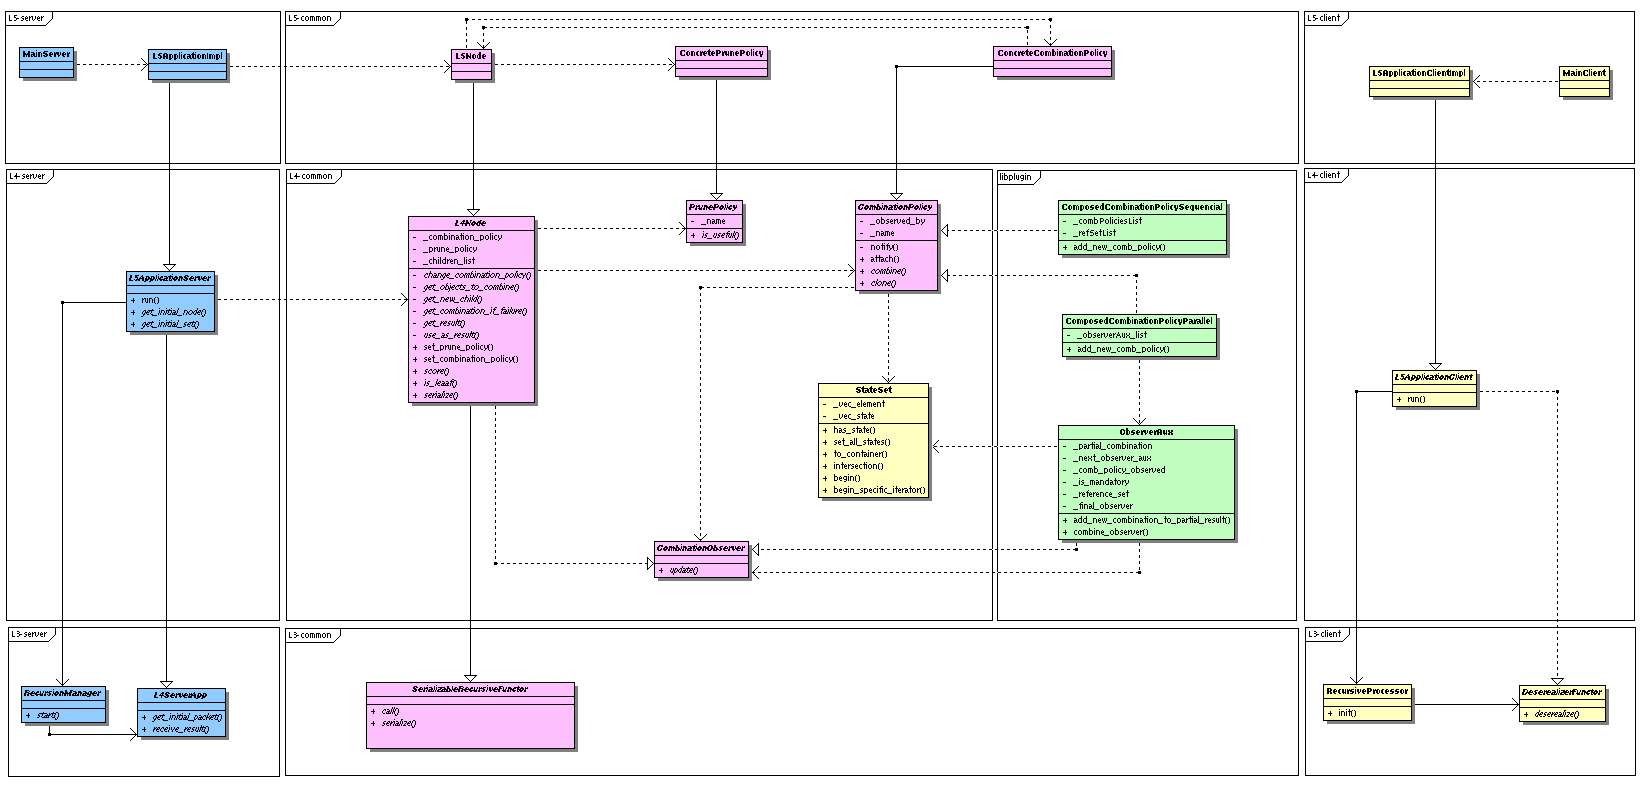
\includegraphics[width=2\textwidth, angle=270]{images/classDiagram.png}
%% 	                \caption{Diagrama de Clases de \combeng \ y sus capas inmediatas}
%% 	                \label{redisenioFud}
%%                 \end{figure}
                \begin{landscape}
               	\begin{figure}
    	            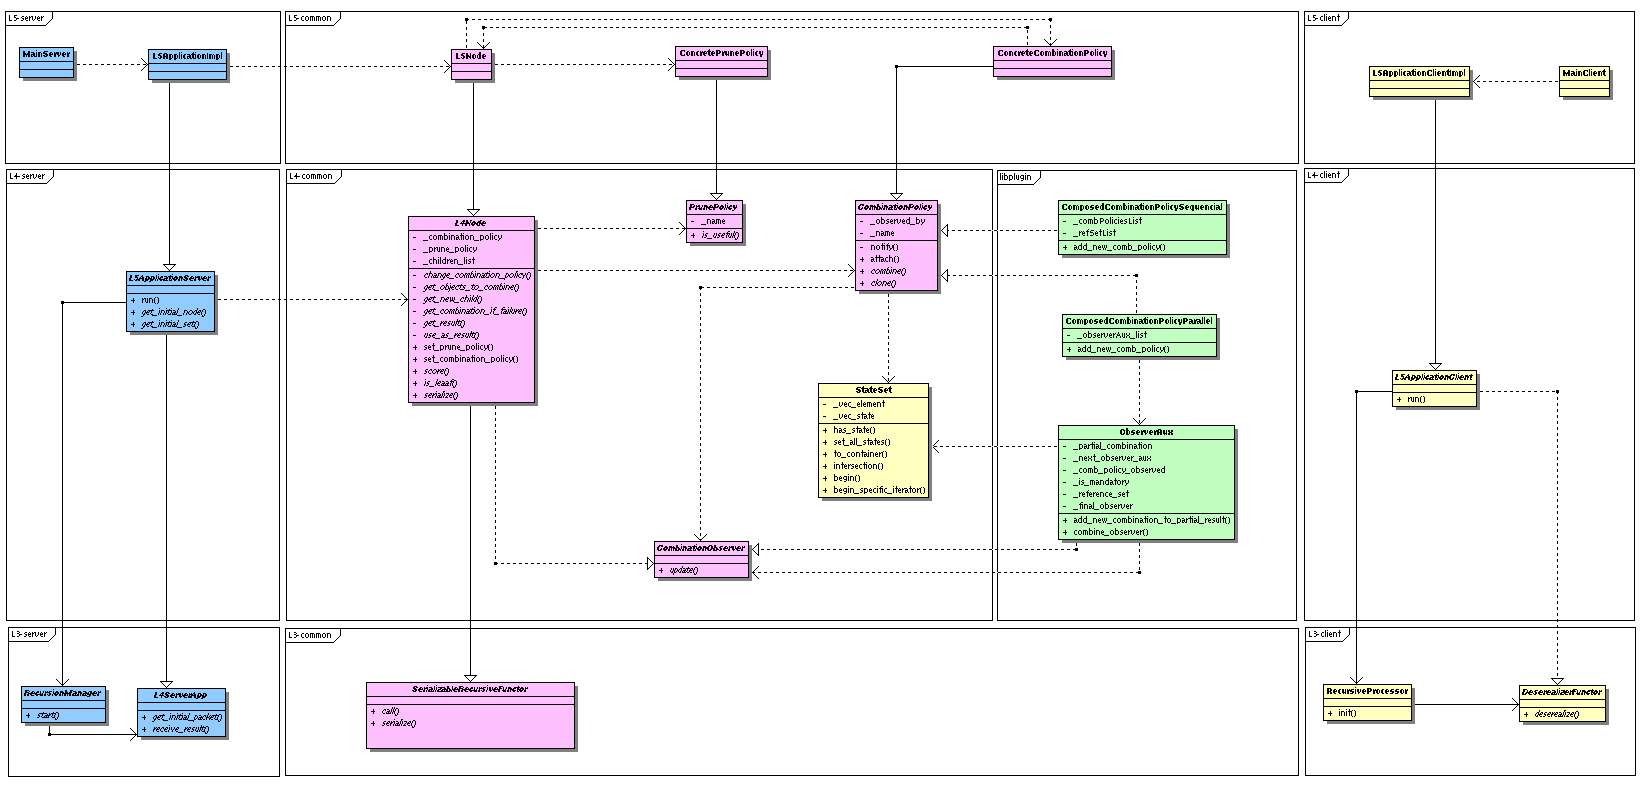
\includegraphics[scale=.36]{images/classDiagram.png}
	                \caption{Diagrama de Clases de \combeng \ y sus capas inmediatas}
	                \label{classDiagram}
                \end{figure}
                \end{landscape}
        	\end{center}
		
	\section{Dise\~no de Bajo Nivel}
		Aqu\'i se hace un refinamiento de las decisiones de dise\~no sobre aquellos componentes abstractos presentes en el dise\~no de 
		alto nivel. Adem\'as, se analiza c\'omo estas clases est\'an compuestas: los atributos de cada una, los m\'etodos que declaran y sus interacciones con el resto del sistema.
		
		Sin entrar en mucho detalle sobre las decisiones de dise\~no que se tuvieron en cuenta sobre cada m\'odulo, se examina, a continuaci\'on, la capa 
		\combeng . Para cada componente del m\'odulo se muestra un diagrama de clases simplificado.
		
		\subsection{\texttt{L4node}}
			En la secci\'on \ref{nodoL4} solo se hab\'ia hecho menci\'on a un nodo de \combeng \ como un concepto abstracto de estado de una aplicaci\'on, pero 
			como se puede observar en la figura \ref{l4NodeClass}, \texttt{L4Node} hereda de \texttt{CombinationObserver} y \texttt{SerializableRecursiveFunctor}, 
			satisfaciendo otros dos roles que se explican a continuaci\'on:
			\begin{itemize}
				\item\textit{L4Node es un observador:} el nodo observa a la pol\'itica de combinaci\'on. 
				Por cada nueva combinaci\'on que la pol\'itica del nodo corriente genere, \'este ser\'a notificado y evaluar\'a, mediante su pol\'itica de poda,
        si dicha combinaci\'on es \'util. En caso afirmativo, crear\'a un nuevo nodo del nivel 5 (de ahora en m\'as lo llamaremos \texttt{L5Node}) y lo
        pondr\'a en su lista de hijos (\texttt{\_children\_list}).
				\item\textit{L4Node es un functor recursivo:} para ello, el nodo del nivel 4 debe implementar los m\'etodos que \texttt
				{SerializableRecursiveFunctor} define en el nivel 3, que son los m\'etodos \texttt{call} y \texttt{serialize}.
				\begin{description}
					\item \footnotesize{\texttt{void serialize(recabs::Packet\& pkt)}}
					
					\normalsize Este m\'etodo, por razones obvias de que el nodo en L4 no posee ning\'un tipo de informaci\'on \'util para la aplicaci\'on, es 
					imposible brindar alg\'un modo de serializaci\'on que resulte de utilidad. Debido a \'esto, quien lo implementa es \texttt{L5Node}.
					
					\item \footnotesize{\texttt{void call(recabs::ChildrenFunctors\& children, recabs::Packet\& result)}}
					
					\normalsize \texttt{call} est\'a implementado usando los m\'etodos virtuales definidos en esta clase, dado que, al igual que la 
					serializaci\'on, en la capa 4 no se tiene informaci\'on suficiente sobre el dominio del problema. En la figura \ref{SDcall} se muestra un 
					diagrama de secuencia exhibiendo el comportamiento de este m\'etodo.
          \begin{figure}[H]\hspace{-.9cm}
    			 	    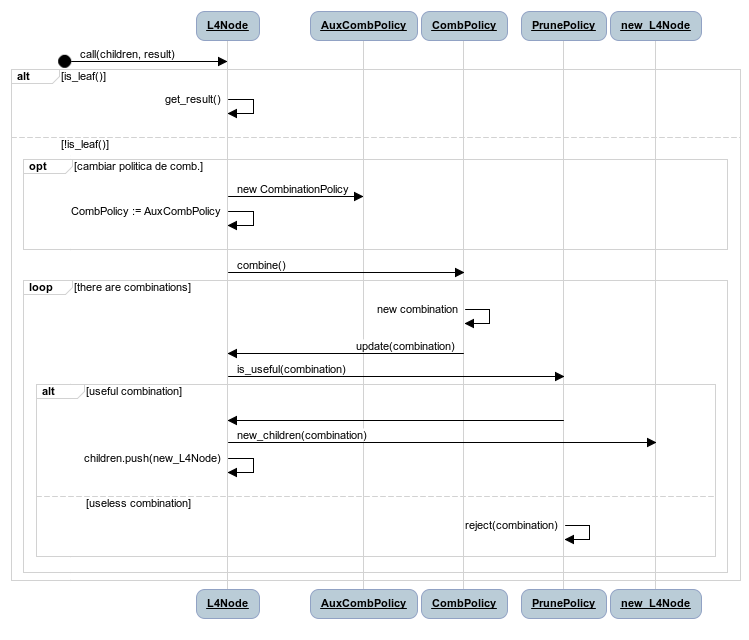
\includegraphics[scale=.6]{images/Call_SeqDiagram.png}
		                \caption{Diagrama de Secuencia del M\'etodo \texttt{call}.}
				    \label{SDcall}
        	\end{figure}
          \vspace{-.6cm}
				\end{description}
				\item \textit{L4Node es un estado de aplicaci\'on:} adem\'as de la serializaci\'on, el desarrollador de la aplicaci\'on debe implementar los 
				siguientes m\'etodos en su L5Node:
				\begin{itemize}
            \scriptsize{}
					\item \texttt{void new\_children(const std::list<T>\&  combination, std::list<L4Node*>\&)}
					\item \texttt{float score()}
					\item \texttt{CombinationPolicy<T>* get\_combination\_if\_failure(const std::string\& failed\_comb\_policy)}
					\item \texttt{CombinationPolicy<T>* change\_combination\_policy()}
					\item \texttt{bool use\_as\_result()}
					\item \texttt{recabs::Packet get\_result()}
					\item \texttt{void get\_objects\_to\_combine(std::list<T>\&)}
					\item \texttt{bool is\_leaf()}
					\item \texttt{void serialize(recabs::Packet\& pkt)}
				\end{itemize}
			\end{itemize}
			\begin{figure}[H] \hspace{.65cm}
    	 	    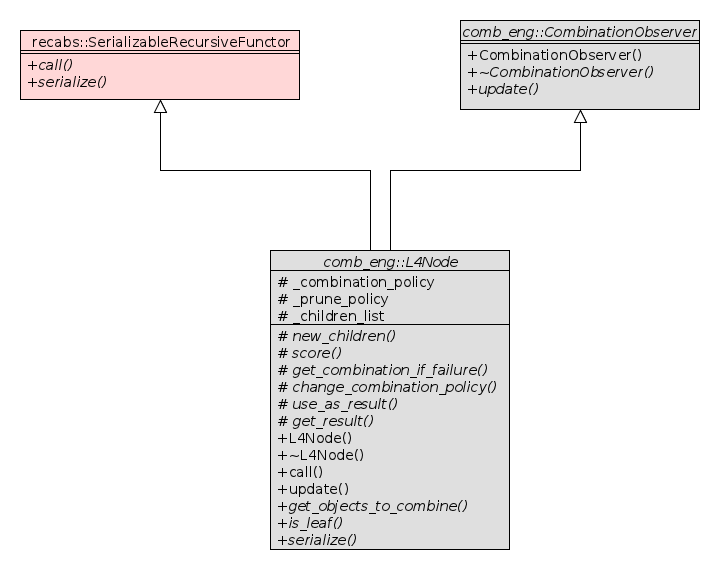
\includegraphics[scale=.46]{images/l4node_class.png}
		        \caption{Clase \texttt{L4Node}.}
		        \label{l4NodeClass}
            \end{figure}

		\subsection{\texttt{PrunePolicy}}
			La pol\'itica de poda es la que define si una combinaci\'on es de utilidad o no. El desarrollador de la aplicaci\'on deber\'a implementar en su 
			pol\'itica de poda concreta el \'unico m\'etodo definido por la interfaz que se observa en la figura \ref{prunePolicyClass}:
			\begin{itemize}
				\item[-] \footnotesize{\texttt{bool is\_useful(const std::list<T>  combination)}}
			\end{itemize}			
			\begin{figure}[H]\hspace{4cm}
   	   	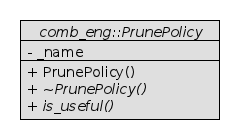
\includegraphics[scale=.56]{images/prune_policy_class.png}
	      \caption{\texttt{PrunePolicy} class}
	      \label{prunePolicyClass}
       \end{figure}

		\subsection{\texttt{CombinationObserver}}
      Para las pol\'iticas de combinaci\'on se utiliz\'o el patr\'on de dise\~no \textit{Observer} (\textit{ve\'ase} \ref{patron_observer}). Como se
      mencion\'o anteriormente, \texttt{L4Node} es un observador de una pol\'itica, por lo que el mismo deber\'a implementar el m\'etodo update
      definido en CombinationObserver:
      \begin{description}
        \item \texttt{void update(const std::list<T>\& combination)}
      \end{description}
				\begin{figure}[H] \hspace{3.6cm}
    	   	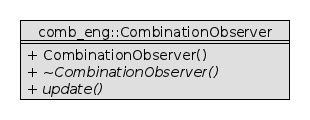
\includegraphics[scale=.56]{images/combination_observer_class.png}
          \caption{Clase \texttt{CombinationObserver}.}
		      \label{combObserverClass}
        \end{figure}
		\subsection{\texttt{CombinationPolicy}}
			La pol\'itica de combinaci\'on es la que define la forma en que una colecci\'on de elementos ser\'an combinados. El desarrollador deber\'a implementar 
			en su pol\'itica de combinaci\'on concreta, los m\'etodos de la interfaz que se observan en la figura \ref{combPolicyClass}:
			\begin{itemize}
				\item[-] \footnotesize{\texttt{void combine(const std::list<T>\&  objects\_to\_combine, Status\& combination\_status)}}. \normalsize{}Como su nombre 
				  lo indica, es el que determina el comportamiento de la pol\'itica, c\'omo se generan las combinaciones. Posee dos argumentos, el primero es la 
				  colecci\'on de elementos que debe combinar y el segundo es el estado con el que finaliza.
				\item[-] \footnotesize{\texttt{CombinationPolicy<T>* clone (CombinationObserver<T>* obs)}}.\\ 
				  \normalsize Retorna una nueva instancia id\'entica a la pol\'itica de combinaci\'on sobre la cual se invoca.
	
			\end{itemize}
			\begin{figure}[ht] \hspace{3.6cm}
    	  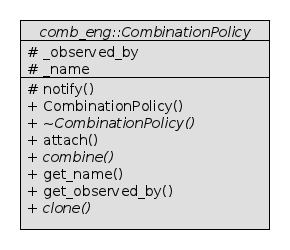
\includegraphics[scale=.56]{images/combination_policy_class.png}
		    \caption{\texttt{CombinationPolicy} class}
		    \label{combPolicyClass}
      \end{figure}
      \subsubsection{Pol\'iticas De Combinaci\'on Provistas Por \combeng}
      	Durante el desarrollo de las aplicaciones que se incluyen en este proyecto se han implementado 
      	diferentes pol\'iticas de combinaci\'on, algunas \textit{simples} y otras \textit{compuestas}. Las simples son algoritmos combinadores propiamente 
      	dichos, mientras que las compuestas combinan a dos o m\'as pol\'iticas simples. Estas \'ultimas no generan combinaciones por s\'i mismas, son las 
      	simples quienes se encargan de obtenerlas.
        		
      	Dentro de las simples, est\'an:
      	\begin{itemize}
          \item \texttt{ListCombinationPolicy}\label{listCombPolicy}: Esta pol\'itica retornar\'a uno a uno los elementos a combinar. El argumento
            \texttt{combination\_status} informar\'a un fallo si el conjunto de elementos se encuentra vac\'io.
      		\item \texttt{NewtonianCombinationPolicy}: el m\'etodo \texttt{combine} de esta pol\'itica implementa el cl\'asico algoritmo que retorna
       			todos los subconjuntos de tama\~no K, con \emph{MIN$\leq$K$\geq$MAX} \footnote{MIN y MAX son establecidos por el usuario}. El \texttt{combination\_status} 
			informa la ocurrencia de un fallo en caso de que la cantidad de elementos a combinar sea sea cero o menor a \emph{MIN}.
       			
      	\end{itemize}
        Mientras que de las compuestas hay otras dos:\label{composedCombinationPolicies}
      	\begin{itemize}
	    		\item \texttt{ComposedCombinationPolicySequencial}: Esta pol\'itica establece una especie de nexo entre diferentes algoritmos combinatorios. 
	     			B\'asicamente, toma un conjunto de combinadores y los hace combinar en secuencia, uno despu\'es de otro. Podr\'ia pensarse como una cola 
	     			(FIFO) de combinadores, el primero en ingresar a la cola es el primero en combinar.
	     				\begin{figure}[H]\hspace{.8cm}
	     					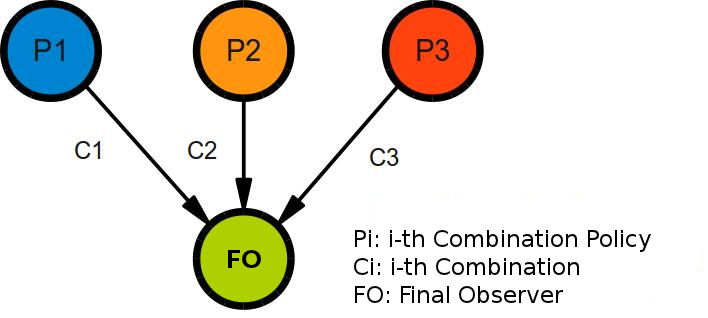
\includegraphics[scale=.45]{images/Comb1.jpg}
	     					\caption{Pol\'itica de Combinaci\'on Compuesta Secuencial.}
	     				\end{figure}
            \item \texttt{ComposedCombinationPolicyParallel}\label{composedCombPolicyParallel}: Esta pol\'itica toma un grupo de algoritmos combinadores
              (pol\'iticas simples) y los pone a ``correr'' en paralelo. Es decir, cada combinaci\'on que genera la primer pol\'itica se une con cada
              combinaci\'on generada por la segunda y as\'i sucesivamente, hasta llegar a la \'ultima de \'estas, la cual har\'a entrega de todo el 
              paquete al observador final.
      			\begin{figure}[H]\hspace{.3cm}
	     				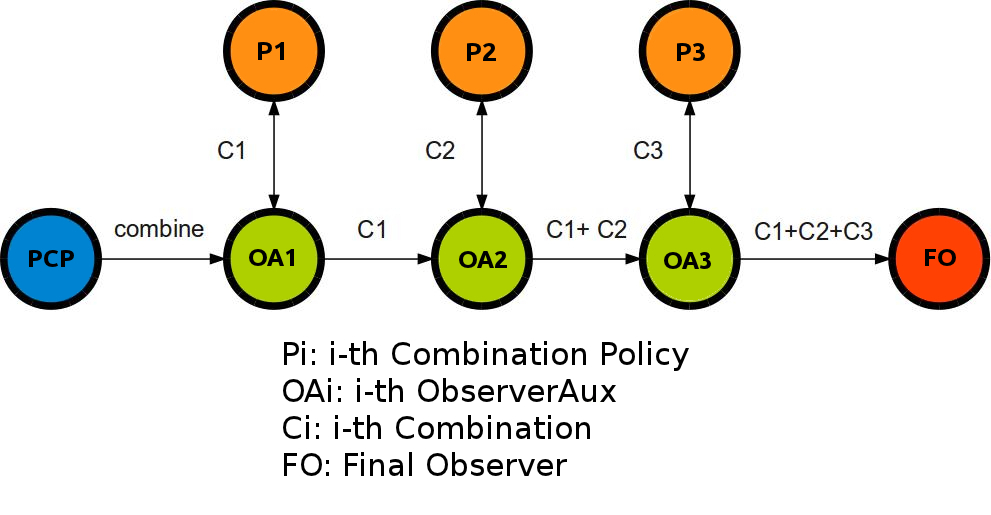
\includegraphics[scale=.4]{images/Comb2.jpg}
	     				\caption{Pol\'itica de Combinaci\'on Compuesta Paralela.}
              \label{parallelComb}
	     			\end{figure}
            \newpage
            De la Figura \ref{parallelComb} se puede observar la nueva entidad \textit{ObserverAux} la cual realiza, repetitivamente hasta que no
            reciba m\'as combinaciones, las siguientes tareas:
            \begin{itemize}
              \item Recibir una combinaci\'on generada por la pol\'itica que observa.
              \item Unir dicha combinaci\'on con aquella que proviene del observador auxiliar anterior, siempre y cuando no se trate del primer
                algoritmo combinatorio (\textbf{P1}). 
              \item Entregar la uni\'on al observador auxiliar de la siguiente primitiva simple. 
            \end{itemize}
            \begin{figure}[H]\hspace{2.8cm}
              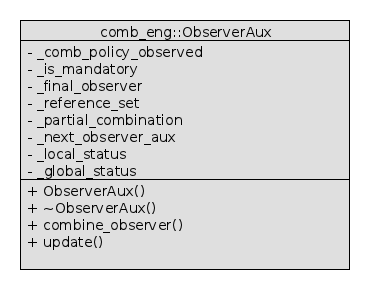
\includegraphics[scale=.6]{images/observer_aux_class.png}
              \caption{Clase \texttt{ObserverAux}.}
              \label{observerAux}
            \end{figure}
            A partir de la figura anterior, se explican cada uno de sus atributos:
            \begin{description}
              \item \texttt{\_comb\_policy\_observed}: tal y como su nombre lo indica, es la pol\'itica a la que se esta observando.
              \item \texttt{\_is\_mandatory}: a la hora de la creaci\'on de una nueva instancia de un ObserverAux, es necesario establecer si la misma ser\'a
                mandatoria o no. Cada una de las pol\'iticas simples opera sobre un conjunto de elementos (\_reference\_set) no necesariamente igual al resto,
                por lo que si una de las pol\'iticas falla (por ejemplo, no dispone de mas combinaciones) y es mandatoria, toda la pol\'itica compuesta
                fallar\'a. Por otro lado, si la misma no es mandatoria implica que este observador auxiliar act\'ue como un ``puente'', dejando
                pasar aquellas uniones que provienen de las primitivas anteriores a siguiente observador.
              \item \texttt{\_partial\_combination}: es la combinaci\'on que recibe del observador auxiliar anterior a \'el. En el caso de que sea el primero,
                este atributo estar\'a vac\'io.
              \item \texttt{\_next\_observer\_aux}: es aquel al que se le debe entregar la combinaci\'on parcial.
              \item \texttt{\_global\_status} y \texttt{\_local\_status} son los que permiten llevar el estado de la pol\'itica compuesta y de cada una de las
                primitivas simples, respectivamente.
            \end{description}
      		\end{itemize}
        	
		\subsection{\texttt{L5ApplicationServer}}
		L5ApplicationServer constituye el lado servidor de la aplicaci\'on. Quien desarrolle una aplicaci\'on sobre \combeng, deber\'a implementar, al menos, los siguientes m\'etodos:
		\begin {description}
		  \item \texttt {get\_initial\_packet}: Retorna un paquete de datos representando al nodo inicial de la aplicaci\'on. Dicho nodo es enviado a un cliente, para que sea \'el quien inicie la ejecuci\'on de la aplicaci\'on.
		  \item \texttt {receive\_result}: Durante el procesamiento de un nodo, los clientes pueden enviar resultados al servidor. Este m\'etodo es quien decide qu\'e hacer con los mismos.
		\end {description}


			\begin{figure}[H] \hspace{3.6cm}
       	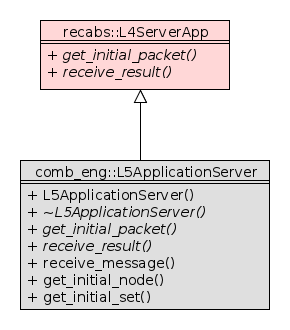
\includegraphics[scale=.56]{images/l5app_server_class.png}
        \caption{Clase \texttt{L5ApplicationServer}.}
        \label{l5AppServerClass}
 	    \end{figure}
        	
		\subsection{\texttt{L5ApplicationClient}}
		L5ApplicationClient constituye el lado cliente de la aplicaci\'on. El desarrollador deber\'a proveer la implementaci\'on de la \'unica funcionalidad requerida por \combeng:
  		\begin {description}
		  \item \texttt {deserialize}: Este m\'etodo efect\'ua el proceso de conversi\'on de un paquete que viaja por la red (\emph {binary-stream}) a un nodo utilizable por la aplicaci\'on. 
		\end {description}


			\begin{figure}[H] \hspace{3.6cm}
        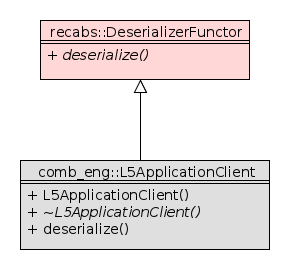
\includegraphics[scale=.56]{images/l5app_client_class.png}
        \caption{Clase \texttt{L5ApplicationClient}.}
        \label{l5AppClientClass}
 	    \end{figure}

\chapter{Implementaci\'on}
  \section{M\'etricas de C\'odigo}
    Para analizar el c\'odigo est\'aticamente se usaron herramientas como Cloc y CCCC. En esta secci\'on se describen m\'etricas de c\'odigo
    generales obtenidas por ambas herramientas y se analizan los resultados obtenidos.

    \subsection{M\'etricas de \combeng}
    \combeng \ esta constituido por 13 archivos de cabecera con un total de 2072 l\'ineas de texto a la fecha de publicaci\'on de
    este documento. La Tabla \ref{clocCombeng} resume los resultados obtenidos despu\'es de correr \textit{cloc} sobre los archivos fuentes de
    \combeng. 
    \begin{table}[!htf]
      \begin{center}
        \begin{tabular}{|l|r|r|r|r|c|}
          \hline
          \multicolumn{2}{|c|}{Files} & \multicolumn{3}{|c|}{Line Types} \\
          \hline
          \textbf{Type} & \textbf{Count} & \textbf{Blank} & \textbf{Comment} & \textbf{Source} \\
          \hline
          \texttt{C++ header} & 13   &  277  &  841  &  947 \\
          \hline
          \textbf{Total}      & 13   &  277  &  841  &  947 \\
          \hline
        \end{tabular}
        \caption{Resultados de cloc para la capa \combeng}\label{clocCombeng}
      \end{center}
    \end{table}
    Los resultados revelan que \combeng \ no es un proyecto de gran tama\~no. Sin embargo, estas medidas no reflejan su complejidad.

    Dijkstra escribi\'o un ensayo muy interesante\cite{ewd1036} donde reflejaba porqu\'e las empresas no deber\'ian considerar las L\'ineas de
    C\'odigo como una medida exacta de la productividad del software. Medir la ``productividad de un programador'' en t\'erminos del 
    ``n\'umero de l\'ineas de c\'odigo que produce por mes'', fomenta la escritura de c\'odigo ins\'ipido.

    Por otro lado, a mayor n\'umero de l\'ineas de c\'odigo, mayor es la complejidad de un producto de software, pero solo en el sentido de que 
    es m\'as dificultoso de mantener y comprender, no tiene relaci\'on directa con la funcionalidad que \'el provee.

    Continuando con los resultados de Cloc, otro dato interesante es la cantidad de l\'ineas de comentarios en el proyecto y su porcentaje con
    respecto al total de l\'ineas del proyecto:

    $$\frac{\#comment\_lines}{\#comment\_lines + \#code\_lines}$$

    Este valor ronda el 0.45, por lo que hay una cantidad de l\'ineas de comentarios similar a las l\'ineas de c\'odigo.
    Para este porcentaje de l\'ineas de comentarios hay una explicaci\'on, y es que incluso archivos realmente peque\~nos incluyen una
    cabecera (``heading'') definiendo ciertos detalles del archivo, como sus autores, fecha de craci\'on y la licencia por cual se rige.

    Todo componente de software (clases, estructuras, funciones, atributos, etc.) conlleva una descripci\'on detallada a ser interpretada por
    \textit{doxygen} (el cual incluye perfiles de funciones) para la generaci\'on de documentaci\'on autom\'atica. La Tabla \ref{comment} muestra un
    ejemplo de la notaci\'on utilizada para doxygen exhibiendo adem\'as el porqu\'e de las m\'etricas de \combeng \ mencionadas anteriormente.

      \begin{table}[!htb]
        \lstset{language=C++}
        \begin{lstlisting}[frame=single]
          /**
          *  It starts the node execution. 
          *  If the current node has some objects available,
          *  it will combine them and the rest of its behaviour
          *  is defined by both combination and prune policies.
          *  The call method tries to fill the node's children list.
          *
          *  @param children : List of children obtained from the excecution of this node.
          *  @param result   : In case that a node wants to send a result to the server,
          *                    it has to fill this parameter with the desired information.
          *  @param when     : it establishes when the result packet has to be sent to 
          *                    the server.
          */>
          void call(recabs::ChildrenFunctors& children, recabs::Packet& result, recabs::WhenToSend& when)
        \end{lstlisting}
        \centering \caption{Comentario de una funci\'on}\label{comment}
      \end{table}

  \subsection{M\'etricas de la Aplicaci\'on \textbf{RNAFoldingFreeEnergy}}
    Los resultados que se obtuvieron para la aplicaci\'on, implementada como la capa m\'as alta del framework, no distan demasiado de aquellos que se
    obtuvieron para \combeng. La aplicaci\'on \rnaffe \ se compone de 12 archivos en total, con una cantidad de 1759 l\'ineas de texto. La
    tabla \ref{clocRnaFFE} resume los resultados obtenidos despu\'es de correr \textit{cloc} sobre los archivos fuentes de \rnaffe.
    
    \begin{table}[!htf]
      \begin{center}
        \begin{tabular}{|l|r|r|r|r|c|}
          \hline
          \multicolumn{2}{|c|}{Files} & \multicolumn{3}{|c|}{Line Types} \\
          \hline
          \textbf{Type} & \textbf{Count} & \textbf{Blank} & \textbf{Comment} & \textbf{Source} \\
          \hline
          \texttt{C++ Header} & 7  &  158  &   442  &    532 \\
          \hline
          \texttt{C++ Source} & 5  &   84  &   245  &    298 \\
          \hline
          \textbf{Total}      & 12 &  242  &   687   &   830 \\
          \hline
        \end{tabular}
        \caption{Resultados de cloc para la capa de aplicaci\'on \rnaffe}\label{clocRnaFFE}
      \end{center}
    \end{table}

    \subsubsection{Cobertura de C\'odigo para \rnaffe}
      La tabla que se muestra a continuaci\'on exhibe la cobertura de c\'odigo de los archivos m\'as relevantes para la aplicaci\'on. Este test de
      cobertura fue realizado ejecutando a la aplicaci\'on \rnaffe \ con la secuencia de pseudo-nucle\'otidos \emph{H2XB} y con los siguientes
      antivirales: \emph{Didanosine, Abacabir, Emtricitabine, Lamivudine, Stavudine, Zidovudine, Tenofovir, Zidovudine, Nevirapine, Efavirenz, Atazanavir, 
      Darunavir, Fosamprenavir, Indinavir, Lopinavir, Nelfinavir, Saquinavir, Tripanavir}.

      \begin{table}[!htf]
        \begin{center}
          \begin{tabular}{|l|r|r|c|}
            \hline
            & \multicolumn{2}{|c|}{Lines of Code} & Percentage \\
            \hline
            \textbf{File} & \textbf{Total} & \textbf{Executed} &  \hspace{1cm}\textbf{\%} \\
            \hline
            \scriptsize{main\_client.cpp} & 17 & 17 & 100 \\
            \hline 
            \scriptsize{main\_server.cpp} & 40 & 24 & 60 \\
            \hline 
            \scriptsize{rnaffe\_application\_client.cpp} & 23 & 23 & 100 \\
            \hline 
            \scriptsize{rnaffe\_application\_server.cpp} & 53 & 53 & 100 \\
            \hline 
            \scriptsize{rnaffe\_node.cpp} & 81 & 57 & 70.37 \\
            \hline 
            \textbf{Total} & 214 & 174 & 81.30 \\
            \hline 
          \end{tabular}
          \caption{Resultados de cobertura para los archivos principales de \rnaffe} \label{rnaffecov}
        \end{center}
      \end{table}
      

\chapter{Aplicaci\'on de Prueba}
Una vez finalizada la tarea de implementaci\'on del motor combinatorio, se continua con la elaboraci\'on de una aplicaci\'on sencilla cuya \'unica
finalidad es la comprobaci\'on de que el motor funcione de la manera esperada.

Esta aplicaci\'on, de nombre \textbf{Clothes Changer}, no requiere distribuci\'on de su trabajo debido a la simpleza en sus c\'alculos, pero a\'un as\'i es
de gran utilidad para poder probar algunas pol\'iticas de combinaci\'on como as\'i tambi\'en observar la nueva capa acoplada a \fud.

\section{Descripci\'on Del Problema}
A partir de un conjunto de prendas de vestir, se desea conocer todas las posibles maneras en que una persona puede vestirlas, es decir, armar todas
las combinaciones del conjunto de ropas. Adem\'as, se quiere hacer un ``ranking'' con las mejores 5 vestimentas.

Cada prenda pertenece a una de las siguientes categor\'ias (notar que una vestimenta es factible siempre y cuando est\'e consituida por una prenda de
cada una de estas categor\'ias).
\begin{itemize}
  \item Pantalones.
  \item Remeras.
  \item Medias.
  \item Calzados.
\end{itemize}

\section{Soluci\'on}
Debido a que la aplicaci\'on fue pensada como un caso de estudio simple para el motor combinatorio, la misma ha sido implementada respetando la interface
que \combeng \ propone. La soluci\'on planteada puede ser descompuesta en dos partes:
\begin{itemize}
  \item Generar todas las posibles vestimentas.
  \item Calcular un puntaje o \textit{score} para cada vestimenta, representando qu\'e tan buena es la combinaci\'on de prendas.
\end{itemize}

\subsection{Generaci\'on De Vestimentas}
Para generar todas las posibles vestimentas se utiliza una pol\'itica de combinaci\'on paralela (ver \ref{composedCombPolicyParallel}), donde cada pol\'itica
simple que la compone es del tipo \emph{ListCombinationPolicy}, cada una actuando sobre una \'unica categor\'ia de ropa.
\begin{center}
  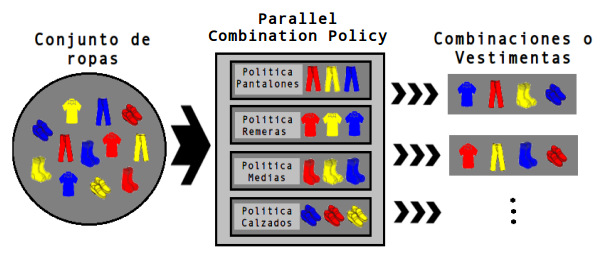
\includegraphics[width=\linewidth]{images/sequencial_ropa.png} 
\end{center}
\newpage
\subsection{C\'alculo Del Score Para Una Vestimenta}
Las tablas que se muestran a continuaci\'on determinan qu\'e tan bien ``combinan'' dos prendas (un pantal\'on con una remera, o un pantal\'on con un
par de medias, etc.). El valor o puntaje de una vestimenta se obtiene realizando la suma entre las diferentes tablas, a partir de las prendas de
vestir que la componen (las tablas fueron inicializadas con valores aleatorios). \\

\textbf{\emph{Tabla Remera-Pantal\'on}}\\

\begin{tabular}{|c|c|c|c|c|}
  \hline Ropa y Color        & Rem. Blanca & Rem. Amarilla      & Rem. Roja  & Rem. Azul \\ 
  \hline Pant. Blanco   & 5           & 2                & 4            &  7          \\
  \hline Pant. Amarillo & 4           & 5                & 6            &  4          \\ 
  \hline Pant. Rojo     & 4           & 4                & 2            &  7          \\ 
  \hline Pant. Azul     & 3           & 5                & 4            &  9          \\  
  \hline 
\end{tabular}

\vspace*{.9cm}
\textbf{\emph{Tabla Pantal\'on-Medias}}\\

\begin{tabular}{|c|c|c|c|c|}
  \hline Ropa y Color      & Pant. Blanco 	   & Pant. Amarillo	     & Pant. Rojo      & Pant. Azul \\ 
  \hline Med. Blancas      & 3           	   & 6               & 9               &  7          \\
  \hline Med. Amarillas    & 5               & 1               & 2               &  9          \\ 
  \hline Med. Rojas        & 4               & 5               & 3               &  1          \\ 
  \hline Med. Azules       & 2               & 4               & 8               &  4          \\  
  \hline 
\end{tabular}

\vspace*{.9cm}
\textbf{\emph{Tabla Medias-Calzados}}\\

\begin{tabular}{|c|c|c|c|c|}
  \hline Ropa y Color      & Med. Blancas & Med. Amarillas      & Med. Rojas & Med. Azules \\ 
  \hline Cal. Blanco    & 6           & 2                & 7            &  1          \\
  \hline Cal. Amarillo  & 3           & 4                & 3           &  2          \\ 
  \hline Cal. Rojo      & 8           & 7                & 6            &  8          \\ 
  \hline Cal. Azul      & 1           & 9                & 2            &  3          \\  
  \hline 
\end{tabular}

\vspace*{.9cm}
A modo de ejemplo, supongamos que una vestimenta generada por el motor combinatorio consta de las siguientes prendas:
\begin{itemize}
  \item \emph{Remera Azul}
  \item \emph{Pantal\'on Blanco}
  \item \emph{Medias Rojas}
  \item \emph{Calzado Blanco}
\end{itemize}
Para calcular el score de esta vestimenta, indexamos las tablas de acuerdo a las ropas que la componen y sumamos los valores. En este caso:

\begin{itemize}
  \item \emph{Remera Azul} y \emph{Pantal\'on Blanco}  = \textbf{7}
  \item \emph{Pantal\'on Blanco} y \emph{Medias Rojas} = \textbf{4}
  \item \emph{Medias Rojas} y  \emph{Calzado Rojo}    = \textbf{6}
\end{itemize}
Dando un valor para la vestimenta de \emph{ \textbf{17}}.

\newpage
\thispagestyle{empty}
\mbox{}
\part{La Aplicaci\'on Rna Folding Free Energy}
\thispagestyle{empty}
\mbox{}
\chapter{Aplicaci\'on Rna Folding Free Energy}\label{RNAFFE_chapter}
% (completar poniendo un ejemplo del archivo de salida)
\section{Motivaci\'on}
En la actualidad, los tratamientos para personas infectadas con HIV consisten de una intensiva terapia antirretroviral. Esta terapia puede ser vista como
una sucesi\'on de aplicaciones de antirretrovirales en el tiempo, donde en cada paso de la sucesi\'on se le suministra al paciente una combinaci\'on
de uno o m\'as antirretrovirales.

Cuando a una persona se le aplica un antirretroviral, el virus comienza a mutar hasta que logra hacerse resistente. \'Esto implica que el antirretroviral
deje de cumplir sus funciones principales y se deba buscar uno nuevo para continuar con el tratamieinto. El orden en que se aplican los antirretrovirales
y c\'omo \'estos son combinados, son factores muy importantes que determinan, entre otras cosas, el tiempo que transcurrir\'a hasta el momento en que el
virus sea resistente a todos los antirretrovirales. 

Hasta el momento, el impacto del escape a los antirretrovirales sobre la estructura secundaria no ha sido estudiada. Esta herramienta pretende recopilar
informaci\'on sobre como var\'ia la Energ\'ia Libre en la estructura secundaria del RNA viral a medida que los antirretrovirales son aplicados sobre
la persona infectada.

\newpage
\section{Soluci\'on}
Para alcanzar el objetivo propuesto, la idea principal puede ser resumida en el siguiente pseudo-algoritmo:
\begin{enumerate}
 \item Tomar una secuencia en representaci\'on del virus y todos los antirretrovirales conocidos hasta el momento.
 \item De todos los antirretrovirales, seleccionar solo aquellos que realmente pueden ser aplicados a la secuencia (un antirretroviral es aplicable
       sobre una secuencia cuando esta \'ultima no presenta resistencia alguna al mismo). De no haber ninguno aplicable, saltar al paso 7.
 \item Generar combinaciones de hasta tres antirretrovirales, utilizando aquellos seleccionados en el paso anterior.
 \item Aplicar cada combinaci\'on de antirretrovirales a la secuencia y obtener todas las secuencias mutantes.
 \item Calcular la FE de cada mutaci\'on.
 \item Ejecutar este proceso para cada una de las mutaciones obtenidas, recibiendo ahora como entrada cada una de esas secuencias mutadas. 
       Luego, saltar al paso 8.
 \item Informar resultado.
 \item Terminar.
\end{enumerate}
Al realizar estos pasos se genera un \'arbol donde cada nodo contiene, entre otras cosas, la secuencia del virus y la energ\'ia libre
(\textbf{FE}) para dicha secuencia. Cabe destacar que una hoja se caracteriza por tener una secuencia a la que ning\'un antirretroviral puede ser aplicado.

Para lograr el objetivo de ver c\'omo el suministro de antirretrovirales afecta la estructura secundaria del RNA viral, basta con seguir los distintos
caminos del \'arbol y observar como var\'ia la FE a medida que avanza la terapia. En la siguiente secci\'on se explicar\'a m\'as detalladamente como
se implement\'o la soluci\'on.

%\begin{figure}[ht]
%\centering
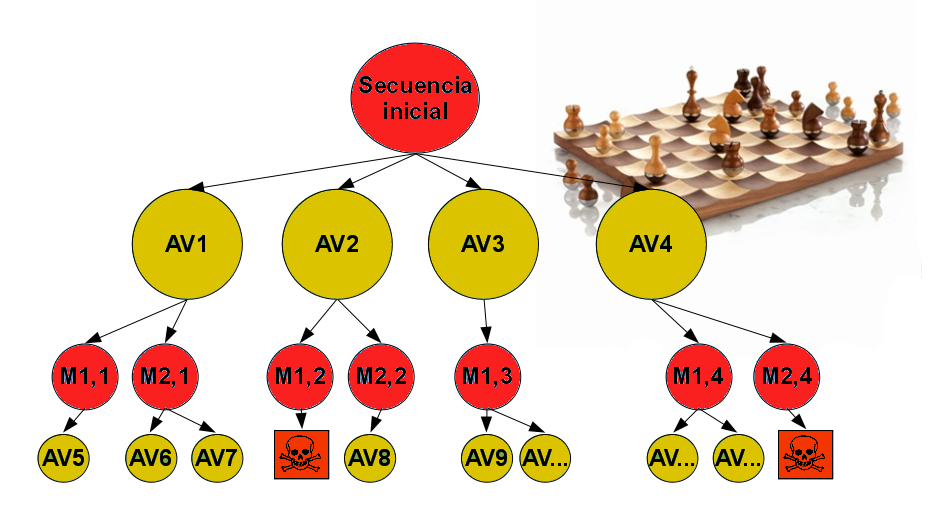
\includegraphics[width=\linewidth]{images/Arbol_ajedrez.png}
%\end{figure} 
En la imagen se muestra como se va generando el \'arbol, los c\'irculos de color rojo representan los nodos y los de color amarillo, los
antirretrovirales que se aplican para obtener la mutaci\'on del nodo hijo. Por otro lado, los recuadros que encierran una calavera establecen que la 
mutaci\'on obtenida es resistente a todos los antirretrovirales, por lo que esas ramas del \'arbol han llegado a su fin.

\section{Implementaci\'on}
En una visi\'on general, como se mencion\'o en otras oportunidades, la soluci\'on consta de armar un \'arbol y analizar los distintos caminos del mismo.
Debido a la gran cantidad de nodos que contiene este \'arbol, a lo costoso que es calcular la energ\'ia libre de una secuencia y a la necesidad de
contar con un motor combinatorio, se decidi\'o implementar la herramienta como la capa de aplicaci\'on del framework \fud. \'Esto nos brinda dos
facilidades imprescindibles:
\begin{enumerate}
 \item La posibilidad de poder realizar los c\'omputos de manera distribuida.
 \item Realizar, eficientemente, las combinaciones de antirretrovirales usando distintas pol\'iticas de combinaci\'on.
\end{enumerate}
  
Seg\'un lo mencionado en \ref{applicationLayer5}, la herramienta constituye el nivel m\'as alto del framework (la capa 5) y debe respetar la API
definida por la capa subyacente, es decir, la capa \textbf{L4-CombinatoryEngine}.
% (imagen de las ultimas dos capas l4, l5. resaltando cual es la interfaz y como se implemento)\\

\subsection{Datos de Entrada}
La herramienta recibe como entrada:
\begin{itemize}
  \item \textit{Secuencia Inicial del Virus}: Archivo que contiene una secuencia de nucle\'otidos representando el ADN del virus.
\begin{lstlisting}[basicstyle=\tt, frame=trBL, tabsize=4,fontadjust=true]
 CCTCAGGTCACTCTTTGGCAACGACCCCTCGTCACAATAAAGGTA
 GATAGGGGGGCAACTAAAGGAAGCTCTATTAGATACAGGAGACGG
 CAGATGATACAGTATTAGAAGAAATGAGTGATTTGCCAGGAA...
\end{lstlisting}
\vspace{.7cm}
 \item \textit{Conjunto de Antirretrovirales}: Archivo .xml conteniendo la base de datos de antirretrovirales.
\begin{lstlisting}[basicstyle=\tt, frame=trBL, tabsize=4,fontadjust=true]
<antivirals>
  ...
  
  <antiviral id="Didanosine" num ="1" type ="tRT" class ="cNRTI">	
    <resistance pos="164" aminos="R"/>
    <resistance pos="173" aminos="V"/>
  </antiviral>

  ...

</antivirals>
\end{lstlisting}

\end{itemize}

\subsection{Representaciones de Datos}
\subsubsection{Secuencia de nucle\'otidos}
Se representa a las secuencias de nucleótidos como cadenas de caracteres. Denotamos a las mismas se denotan como expresiones regulares.
\begin{itemize}
\item $nuc\_arn = a \vert u \vert c \vert g \vert \_$
\item $nuc\_adn = a \vert t \vert c \vert g \vert \_$
\end{itemize} 
Al igual que los nucle\'otidos, se representan los genes de ADN y ARN.
\begin{itemize}
\item $gen\_arn = (nuc\_arn)^{+}$
\item $gen\_adn = (nuc\_adn)^{+}$	
\end{itemize}

\subsubsection{Antirretrovirales}
Un Antirretroviral consta de, principalmente, un listado de posiciones de resistencia. Estas posiciones establecen en qu\'e mol\'eculas del virus
el antirretroviral se comporta de manera efectiva. En el dise\~no propuesto, estas posiciones no son s\'olo m\'s que un par $<pos , aminos>$ donde 
$pos \geq 0$ y $aminos$ es una lista de amino\'acidos. Es decir, la posici\'on de la resistencia describe un valor entero en el cual los amino\'acidos
act\'uan sobre el virus.
%\begin{figure}[h!]
  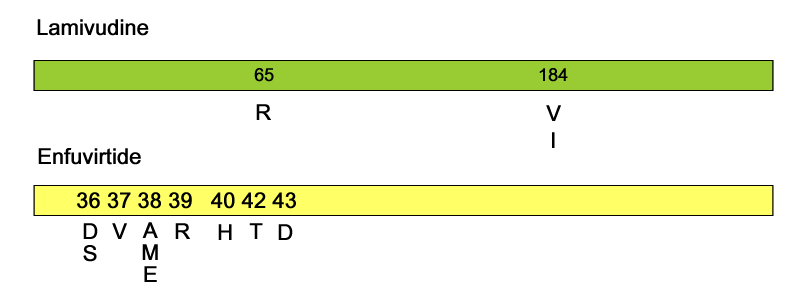
\includegraphics[scale=1]{images/Antivirals.png}\\
%  \caption{Ejemplo de dos antirretrovirales.} 
%\end{figure}

Adem\'as de este listado de posiciones, se incluye otro tipo de informaci\'on para el antirretroviral, como un identificador, un nombre, una clase y
un tipo.

\subsection{Predicci\'on de la Estructura Secundaria}
Esta predicci\'on consiste en obtener la \emph{estructura secundaria} a partir de la estructura primaria (ver \ref{estructuraSecundariaARN}). Existen
dos tipos de algoritmos para realizar esta tarea:
\begin{itemize}
 \item \textbf{Predicci\'on por \emph{minimal free energy (mfe)}}: Propuesto e implementado por Michael Zuker en el a\~no 1981 \cite{Zuker84}, utiliza programaci\'on
   din\'amica para encontrar la estructura secundaria que minimiza la energ\'ia libre.
 \item \textbf{Predicci\'on comparativa}: Utiliza diferentes m\'etodos para comparar secuencias y estructuras con el fin de obtener una estructura por ``consenso''\cite{Gardner04}.
\end{itemize}

Si bien la \textit{predicci\'on comparativa} presenta un incremento en la fidelidad de los resultados obtenidos con respecto a la \textit{predicci\'on
por mfe}, el primer tipo de predicci\'on requiere la existencia de un conjunto de secuencias relacionadas entre s\'i (hom\'ologas) y \'esto no siempre
es posible. En particular, en este trabajo s\'olo interesa poder realizar predicciones de la estructura secundaria a partir de una sola secuencia, por
lo que la predicci\'on comparativa fue descartada.

Entre las implementaciones de la predicci\'on por mfe, se destacan \textbf{RNAfold}\cite{Hofacker94} y \textbf{Mfold}. Ambas implementan el algoritmo propuesto por Michael
Zuker con complejidad $\mathcal{O}(N^{3})$ donde $N$ es la longitud de la secuencia.
A continuaci\'on se puede ver un ejemplo de una predicci\'on realizada con \textbf{RNAfold}.

\begin{verbatim}
combeng@fudepan:~$ RNAfold

  Input string (upper or lower case); 
  ....,....1....,....2....,....3....,....4...
  AAAGGCAACGGCCAU
  length = 15
  AAAGGCAACGGCCAU
  ...(((....)))..
  minimum free energy =  -4.40 kcal/mol
\end{verbatim}

El resultado obtenido es, precisamente, la energ\'ia libre y la estructura secundaria representada con par\'entesis y puntos. Donde los pares de
par\'entesis indican las bases ``apareadas'' o ``unidas'' y los puntos, las bases libres. Para este trabajo, solo es relevante la energ\'ia libre.

\subsection{Selecci\'on de los Antirretrovirales a Aplicar}
  Como se muestra en la siguiente secci\'on, cada nodo del \'arbol de ejecuci\'on dispone de una secuencia de nucle\'otidos. Para saber qu\'e 
  antirretrovirales combinar y as\'i avanzar en la terapia, es necesario obtener de la base de datos de antirretrovirales s\'olo aquellos a los que
  la secuencia del nodo no es resistente. Adem\'as de la condici\'on anterior, se seleccionan, preferentemente, aquellos que representen m\'as
  obst\'aculos para el virus, logrando que al mismo le sea m\'as costoso volverse resistente.\footnote{Para una explicaci\'on m\'as detallada,
  examinar el cap\'itulo 6 de ASO (\url{http://aso.googlecode.com})}
\newpage
\subsection{Preferencia en Combinaci\'on de Antirretrovirales}
Los antirretrovirales individualmente no suprimen la infecci\'on por VIH a largo plazo, por lo cual, actualmente se usan combinaciones de \'estos.
Las combinaciones de antirretrovirales act\'uan incrementando el n\'umero de obst\'aculos para la mutaci\'on viral, manteniendo bajo el n\'umero de
copias virales. En la figura \ref{antivirals_fsm} se muestra una M\'aquina de Estados Finita, de ahora en adelante FSM (por su acr\'onimo en
ingl\'es), representando c\'omo los antirretrovirales son combinados de acuerdo a la disponibilidad de los mismos. Como se explic\'o anteriormente, 
hay tres tipos de antirretrovirales (\textbf{NRTI}, \textbf{NNRTI}, \textbf{PI}). Dependiendo de la cantidad de cada uno que pueden ser aplicados a
la secuencia del nodo corriente, se escoge una pol\'itica de combinaci\'on seg\'un se detalla en la figura.

\begin{figure}[ht]
  \centering
  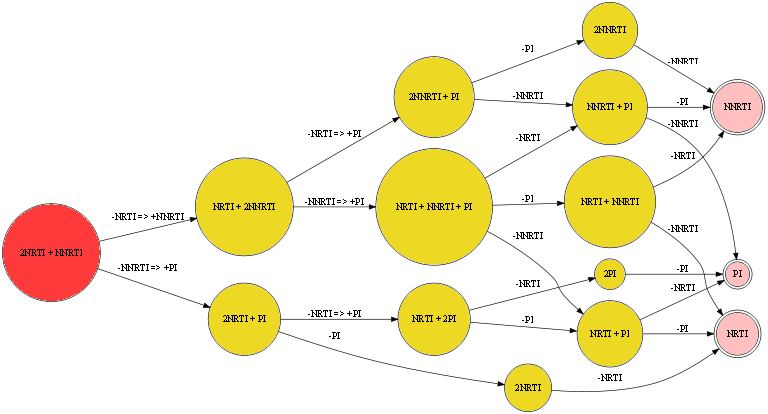
\includegraphics[width=\linewidth]{images/Antivirals_fsm.png}
  \label{antivirals_fsm}
\end{figure}

A modo de ejemplo supongamos que:
\begin{itemize}
 \item  El nodo ra\'iz del \'arbol contiene la secuencia inicial del virus, ll\'amese \textbf{X}.
 \item  Hay m\'as de dos antirretrovirales de cada tipo que se pueden aplicar a la secuencia \textbf{X}.
 \item  La pol\'itica de combinaci\'on del nodo ra\'iz es la representada por el primer estado de la FSM, \textbf{2NRTI+1NNRTI}.
\end{itemize}
Para este caso, la herramienta generar\'a todas las combinaciones de tres antirretrovirales, conteniendo dos del tipo \textbf{NRTI} y uno del tipo
\textbf{NNRTI}. Luego, por cada mutaci\'on obtenida al aplicar una combinaci\'on, se genera un hijo y se le ordena que se ejecute con la misma 
pol\'itica de combinaci\'on. En el momento en que el hijo debe ser ejecutado pueden ocurrir dos cosas:
\begin{enumerate}
 \item La cantidad de antirretrovirales de cada tipo que se le pueden aplicar a la mutaci\'on es suficiente para aplicar la misma pol\'itica de
   combinaci\'on del nodo padre.
 \item La cantidad de antirretrovirales de cada tipo que se le pueden aplicar a la mutaci\'on no es suficiente para aplicar la pol\'itica de 
   combinaci\'on del padre. En este caso, dependiendo del tipo del antirretroviral cuya cantidad es insuficiente, se cambia la pol\'itica de
   combinaci\'on para ejecutar el nodo. Estos cambios se realizan acorde a la FSM mostrada.
\end{enumerate}
%COMPLETAR: ACA TENDRIA QUE PONER XQ DANIEL HIZO ESA FSM.. PORQUE CONVIENE ELEGIR LOS ANTIVIRALES DE ESA FORMA

\subsection{Generaci\'on de Mutaciones a Partir de un Conjunto de Antirretrovirales}
Un antirretroviral esta compuesto, entre otras cosas, por un conjunto de resistencias. Suponga que, a modo de ejemplo, se toma el antirretroviral
Abacavir, el cual tiene como una de sus resistencias el amino\'acido \textbf{R} en la posici\'on \textbf{65}.

\begin{figure}[H]
  
\includegraphics[width=\linewidth]{images/abacadir.png}
\end{figure}

Luego, si el triplete n\'umero \textbf{65} de la secuencia codifica el amino\'acido \textbf{R}, significa que dicha secuencia es resistente a tal antiviral.

\begin{figure}[H]
  
\includegraphics[width=\linewidth]{images/secuencia.png}
\end{figure}
En este caso, el triplete \textbf{ATT} codifica el amino\'acido \textbf{R}, lo cual hace a la mutaci\'on resistente al antirretroviral Abacavir.\\
Para lo obtenci\'on de las mutaciones a partir de un conjunto de antirretrovirales, se desarroll\'o un algoritmo que puede ser resumido en los siguientes pasos:
\newpage
\begin{enumerate}
  \item  Obtener el producto cartesiano de las resistencias de cada antirretroviral. Suponga el siguiente ejemplo,

    \textbf{Antirretrovirales}:
    \vspace{-.5cm}
    \begin{center}
      \emph {A = \{(1,G), (2,T)\}}
    
      \emph {B = \{(3,G), (2,T), (4,R)\}}
     \end{center}
      \scriptsize{En un par \emph{(X, Y)}: \emph{X} representa la posici\'on de la resistencia e \emph{Y} el amino\'acido al cual es resistente.}

      \normalsize{}Luego, el producto cartesiano entre \emph{A} y \emph{B} es:

  \emph{A} x \emph{B =} \vspace{-1cm}
                       \begin{center}
                          \emph{\{\{(1,G), (3,G)\}, \{(1,G), (2,T)\}, \{(1,G), (4,R)\}, \\
                          \{(2,T), (3,G)\}, \{(2,T), (2,T)\}, \{(2,T), (4,R)\}\}}
                       \end{center}
  \item  Aplicar las siguientes reglas a cada subconjunto \emph {S} del producto cartesiano:
      \begin{enumerate}
       \item Si $\exists(x,y),(z,w)\in\emph{S}$ : $x=z$  $\wedge$  $y\neq w$  $\mapsto$  Eliminar \emph{S} del producto cartesiano
         \footnote{Esto se debe a que no existen secuencias en las que para una posici\'on haya dos amino\'acidos.}.

       \item Si $\exists(x,y),(z,w)\in\emph{S}$ : $x=z$  $\wedge$  $y=w$  $\mapsto$  Eliminar una de las repeticiones de \emph{S}.
      \end{enumerate}
     	Una vez aplicadas las reglas, el producto cartesiano del paso anterior queda reducido a:
      
      \emph {A} x \emph{B' =} \vspace{-1cm}
      \begin{center}
         \emph{\{\{(1,G), (3,G)\}, \{(1,G), (2,T)\}, \{(1,G), (4,R)\}, \\
                \{(2,T), (3,G)\}, \{(2,T)\}, \{(2,T), (4,R)\}\}}
         \footnote{S\'olo se aplic\'o la regla del inciso b).}
      \end{center}

    \item  A partir del conjunto obtenido en el paso anterior (\emph{A} x \emph{B'}), se crea un nuevo conjunto (\emph{T}) conteniendo aquellos 
      subconjuntos de \emph{A} x \emph{B'} que tengan la menor cantidad de elementos.

   Es decir, 
   \begin{center}
     Sea \emph{S$_{1}$...S$_{n}$} $\in$ A x B' : \emph{S}$_{i}\in$ T \textbf{Sii} $\forall$\emph{S}$_{j}\in$S : \emph{count}(S$_{i}$) $\leq$ \emph{count}(S$_{j}$).
   \end{center}
   \vspace{-.33cm}
   \scriptsize{(\textit{count}: funci\'on que toma un conjunto y retorna su cantidad de elementos)}

   \normalsize{}Continuando con el ejemplo, \emph{A} x \emph{B'} se reduce a:
   \begin{center}
     \emph{A} x \emph{B' = \{\{(2, T)\}\}}
   \end{center}

  \item  Por cada subconjunto S$_{i}$ del conjunto obtenido en el paso anterior, se obtiene una mutaci\'on. Esto se logra reemplazando en la 
    secuencia de entrada (no mutada), cada una de las resistencias de S$_{i}$.

    En el ejemplo anterior, debido a que hay un \'unico conjunto con m\'inima cantidad de elementos, se obtendr\'a solamente una mutaci\'on. La misma 
    ser\'a el resultado de reemplazar el amino\'acido que haya en la posici\'on \emph{2} de la secuencia de entrada, por \emph{T}.
\end{enumerate}

  Es importante notar que todas las mutantes obtenidas al aplicar un conjunto de antirretrovirales a una secuencia, son resistentes todos los
  antirretrovirales del conjunto.

\subsection{El nodo RNAFFE}
  Los nodos del \'arbol est\'an formados principalmente por:
 \begin{itemize}
  \item La secuencia corriente del virus: representa el ADN corriente del virus.
  \item Pol\'itica de combinaci\'on: Especifica la manera en que van a ser combinados los antirretrovirales.
  \item La terapia que se ha aplicado hasta el momento. Es decir, el nodo contiene una lista de conjuntos de antirretrovirales representando cuales
    han sido aplicados y en que orden se aplicaron los antirretrovirales que llevaron a obtener la secuencia mutante corriente.
  \item Lista de FE's: Su objetivo es almacenar la informaci\'on de como vari\'o la energ\'ia libre a medida que se avanz\'o en la terapia.
 \end{itemize}

\subsection{Obtenci\'on de Los Hijos Para Un Nodo}
Debido a que para obtenci\'on de las distintas combinaciones de antirretrovirales se utiliz\'o el patr\'on de dise\~no \textit{Observer}\footnote{Para
mayor informaci\'on, puede consultar \ref{patron_observer}}, cada vez que una combinaci\'on es generada, el nodo es notificado con dicha combinaci\'on.
Ante tal evento, el nodo reacciona de la siguiente manera:
\begin{enumerate}
  \item  Utilizando su secuencia y la combinaci\'on de antirretrovirales, obtiene una lista de secuencia mutantes, las cuales son resistentes a cada uno
    de los antirretrovirales de la combinaci\'on.
  \item  Con cada secuencia mutante se crea un hijo, al cual se le adjunta la nueva combinaci\'on de antirretrovirales como un paso m\'as en la terapia.
    En este punto es calculada la \textbf{FE} de la mutaci\'on.
\end{enumerate}
 
\subsection{Fallo Virol\'ogico}
En \ref{fracasoTerapeutico} se observ\'o la utilidad del t\'ermino ``fallo virol\'ogico'' en el campo de la medicina. Un fallo virol\'ogico tiene
lugar como resultado de una mixtura poco certera entre una mala adherencia al tratamiento y el desarrollo de resistencias.

En la aplicaci\'on, el t\'ermino es utilizado para especificar esto \'ultimo, la resistencia del virus. Suponga el caso en que se est\'en
combinando dos antirretrovirales de tipo NRTI con uno de tipo NNRTI. Ahora bien, al aplicar una posible combinaci\'on (2\textbf{NRTI}+1\textbf{NNRTI})
se obtiene una secuencia de mutantes. Continuando con la supuesta ejecuci\'on, por cada una de las mutantes se debe crear un nodo hijo, pero antes se
consulta con qu\'e pol\'itica de combinaci\'on debe ser creado. Esto se debe a que puede ser posible que que sobre una de las mutantes ahora s\'olo un
antirretroviral del tipo NRTI sea aplicable, lo que implica que la pol\'itica de combinaci\'on que se utilizaba antes ya no es viable. Luego, el
nuevo nodo hijo dispondr\'a de otra pol\'itica de combinaci\'on para la generaci\'on de sus mutantes acorde a la FSM (v\'ease \ref{antivirals_fsm}).

\subsection{Datos De Salida}
La salida obtenida tras una ejecuci\'on de la herramienta, es un archivo conteniendo cada camino del \'arbol. Dicho de otra forma, el archivo contiene
todas las terapias posibles, adem\'as de mostrar c\'omo fue variando la energ\'ia libre en cada paso de dichas terapias. Este archivo, es utilizado por
R para generar los res\'umenes estad\'isticos necesarios (gr\'aficos, tendencias, etc).
 

\section{Dependencias Externas}
En esta secci\'on se mencionan las dependencias de la aplicaci\'on. La mayor\'ia de ellas pertenecen a \fudepan. Adem\'as, dos nuevas bibliotecas
fueron desarrolladas, ambas como parte de este trabajo final.

\begin{itemize}
  \item \textbf{Biopp}: Biblioteca C++ para Biolog\'ia Molecular. Esta biblioteca es la que provee las estructuras de datos y m\'etodos para
    manipular secuencias de nucle\'otidos. Adem\'as, se realizaron ciertas extensiones para este trabajo, particularmente la
    serializaci\'on/deserializaci\'on de ciertas estructuras utilizadas. Para m\'as informaci\'on, visite el sitio web de la misma, \url{biopp.googlecode.com}.
  \item \textbf{Fx-parser}: FXP es un parser XML de alto nivel para C++. De hecho, FXP es un adaptador de datos que se sit\'ua por encima de un parser
    SAX (Simple API for XML Parsing). Utilizado para parsear el archivo .xml que contiene la base de datos de
    antivirales\footnote{\url{fx-parser.googlecode.com}}.
  \item \textbf{GetOpt\_pp}: GetOpt forma parte de la \textit{glibc} (The GNU C Library). La funci\'on GetOpt provee un mecanismo estructurado y eficiente para
    procesar opciones por l\'inea de comandos para un programa de aplicaci\'on. El proyecto GetOpt\_pp es una otra versi\'on de lo antes mencionado, escrita en C++
    y pertenece a \fudepan. (\url{getoptpp.googlecode.com}).
\end{itemize}

\subsection{Nuevas Bibliotecas}
Para lograr una mejor modularidad en la aplicaci\'on \emph{RNAFoldingFE} fueron creadas dos bibliotecas: Antivirals y RnaFolding. La mayor\'ia de
c\'odigo de ambas bibliotecas es c\'odigo perteneciente a otros proyectos de la fundaci\'on. El trabajo aqu\'i realizado fue el de agrupar el
contenido relevante para este trabajo, como as\'i tambi\'en extenderlo, proveyendo funcionalidades de gran necesidad
(serializaci\'on/deserializaci\'on de ciertas clases, optimizaciones, correcciones, etc.)

\begin{itemize}
  \item \textit{Antivirals}: Define todas las estructuras de datos y m\'etodos para la manipulaci\'on de secuencias de nucle\'otidos y antirretrovirales, como
    aplicar un conjunto de \'estos sobre una secuencia y asi obtener sus mutantes, la carga de la base de datos de antirretrovirales, entre otras. El
    proyecto \textbf{ASO} es qui\'en provey\'o la mayor parte del c\'odigo existente en la biblioteca. Para m\'as informaci\'on acerca de ASO, puede
    consultar \url{aso.googlecode.com}.
  \item \textit{RnaFolding}: Provee, entre otras, las funcionalidades necesarias para obtener la energ\'ia libre de una secuencia de nucle\'otidos.
    Casi la totalidad de su c\'odigo proviene del proyecto \textbf{VAC-O}. Al igual que el proyecto anterior, puede consultar su c\'odigo, su
    documentaci\'on, sus resultados en la URL \url{vac-o.googlecode.com}.
\end{itemize}
Estas bibliotecas, adem\'as de ser necesarias para nuestra tesis, ser\'an utilizadas por futuros proyectos de la fundaci\'on.

\newpage
\section{Resultados}
La herramienta fue ejecutada utilizando los antirretrovirales de la base de datos de la \textit{International AIDS
Society}\footnote{\url{www.iasusa.org}}\cite{JBB08} del a\~no 2010 y, como secuencia inicial, la secuencia HXB2 en representaci\'on del virus. 
Cabe destacar que s\'olo el 50 por cierto de los caminos del \'arbol fueron computados dada a la escasez de recursos computacionales con los que se contaba.

Los resultados aqu\'i presentes fueron obtenidos utilizando el lenguaje y entorno para computaci\'on estad\'istica y gr\'aficos conocido como
\textbf{R}\footnote{\url{www.r-project.org}}. Todos ellos tuvieron como entrada de datos el archivo de resultados originado durante la ejecuci\'on de la aplicaci\'on.

\subsection{Promedio de Longitud de Terapia}
  Esta estad\'istica representa la cantidad de fallos virol\'ogicos que ocurrieron hasta que el virus se hizo resistente a todos los antirretrovirales.
  Dependiendo de c\'omo vaya mutando el virus, var\'ia la longitud de la terapia.
  
  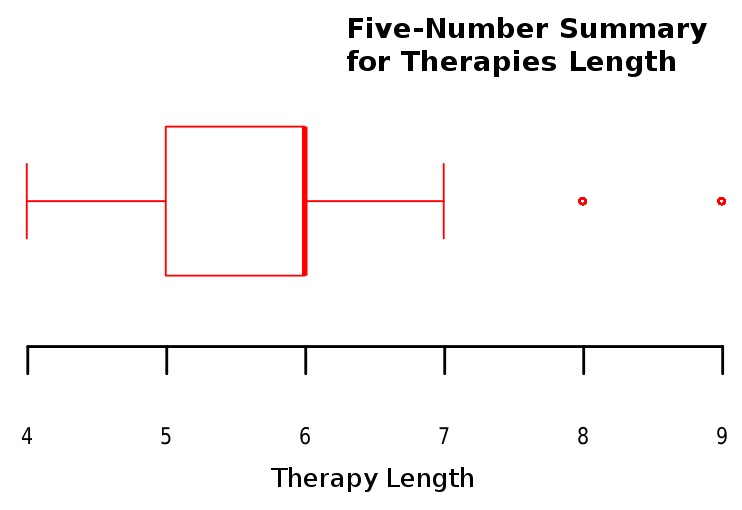
\includegraphics[width=\linewidth]{images/therapy_length.png}
  El gr\'afico revela que la mayor\'ia de las terapias tienen longitud 6 y otra gran cantidad tienen como longitud, 5. Con una menor frecuencia se
  encuentran las terapias con longitudes de 6 y 7, mientras que en muy pocos casos, las mismas alcanzaron valores de 8 o 9. La importancia de estas 
  estad\'isticas residen en el hecho de que mientras m\'as larga es la terapia, m\'as tiempo el paciente podr\'a ser mantenido bajo tratamiento, inhibiendo 
  as\'i el desarrollo de la enfermedad.

\subsection{Sobre la Energ\'ia Libre de las Mutaciones en Relaci\'on a la Longitud de Terapia}
  Cuando un antirretroviral es aplicado, la secuencia de nucle\'otidos que representa el ADN del virus sufre una modificaci\'on, es decir, se produce una
  secuencia mutante y su Energ\'ia libre var\'ia. La idea de este resumen estad\'istico es mostrar c\'omo la energ\'ia libre de las mutaciones se
  incrementa o decrementa acorde se avanza sobre la terapia.\\
  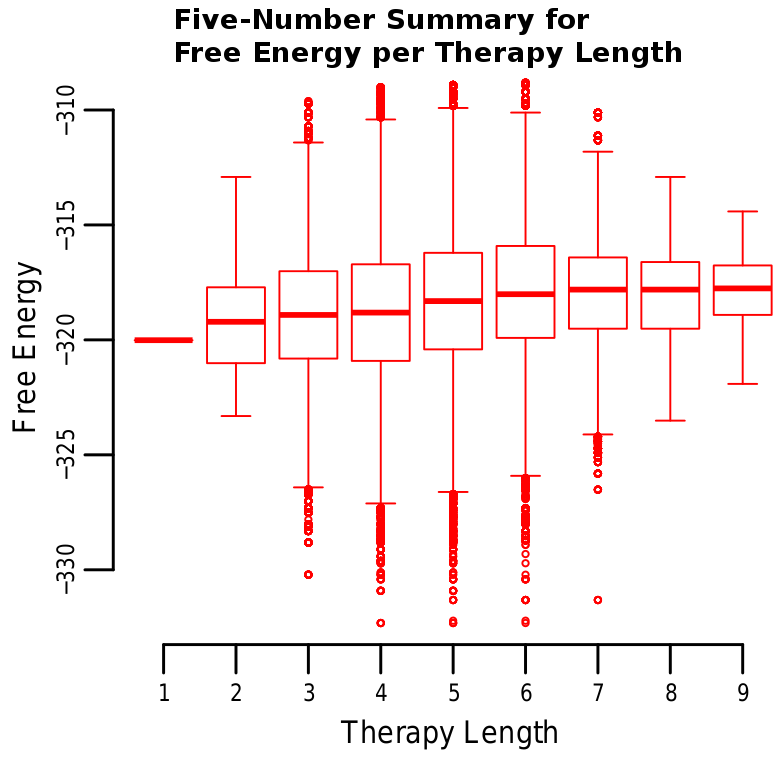
\includegraphics[width=\linewidth]{images/free_energy_by_thrapy_length.png}\\
  Tal y como se puede observar en el gr\'afico, a medida que se avanza en las terapias, los valores promedio para la energ\'ia libre se incrementan
  de manera moderada. Si bien estas variaciones son peque\~nas, las mismas informan que, en la mayor\'ia de los casos, a lo largo de un tratamiento
  el virus sufre cierta desestabilizaci\'on.

\subsection{Estimaci\'on de Tendencia de la Energ\'ia Libre}
  Los datos representados en el siguiente gr\'afico no var\'ian respecto del punto anterior, la \'unica diferencia es que se exhiben de otra manera.
  Esto se realiz\'o para obtener informaci\'on acerca de la tendencia\footnote{\url{www.en.wikipedia.org/wiki/Trend\_estimation}} de la energ\'ia libre a medida 
  que se van aplicando los antirretrovirales de la terapia.\\

  \begin{figure}[H]\hspace{-2cm}
    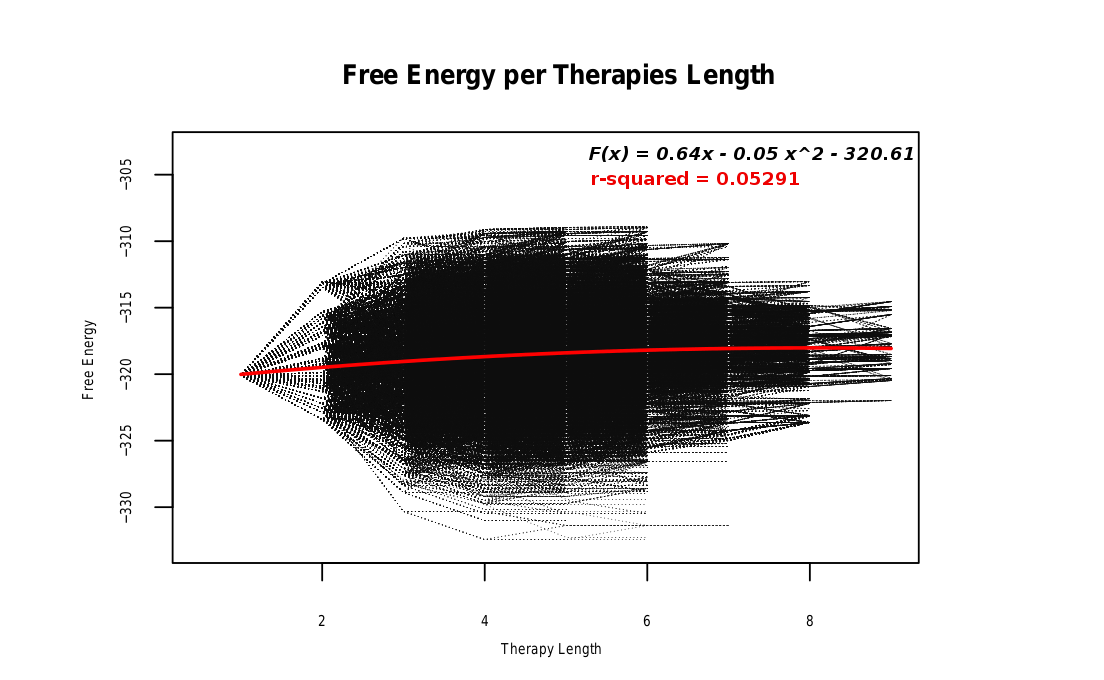
\includegraphics[scale=0.47]{images/ffe_vs_thLength.png}
  \end{figure}
    Como muestra el gr\'afico, los datos se encuentran de manera dispersa. La l\'inea roja que cruza el gr\'afico de nubes representa la tendencia. La
  f\'ormula de dicha l\'inea esta dada por la ecuaci\'on:\\ 
  \newline
  \emph{Y = 0.64X + -0.05$X^{2}$ - 320.61} \\ 
  \newline
  y su $R ^{2}$ es de 0.05291. Si bien el $R ^{2}$ es peque\~no, lo cual significa que
  la ecuaci\'on no aproxima con gran exactitud, se esperan obtener resultados m\'as precisos cuando la herramienta compute el \'arbol de ejecuci\'on
  de manera completa.

\chapter{Conclusiones}
Como resultado de este trabajo se ha obtenido una nueva capa para el framework \fud, de nombre \combeng. La misma ha cumplido con todas las
expectativas y ha cubierto cada uno de los requerimientos planteados desde un comienzo. Si bien s\'olo se ha desarrollado una aplicaci\'on relevante,
y algunas otras como prueba, se puede concluir que el motor combinatorio se encuentra apto para resolver cualquier problema que requiera de
la combinaci\'on de cualquier tipo de elementos. Aquellas aplicaciones que hacen un uso correcto del framework \fud \ y, por ende, de la nueva capa,
no deber\'an preocuparse por asuntos relacionados a la programaci\'on paralela. Esto permite realizar el procesamiento de las
 combinaciones, muchas veces de gran costo computacional, de manera distribuida y sin la necesidad de tener grandes conocimientos en el \'area. 

En cuanto a la aplicaci\'on \rnaffe, se han obtenido numerosos y valiosos datos que hasta el momento no eran conocidos. Tanto la
aplicaci\'on como los datos recolectados recibieron buenas cr\'iticas tras ser presentados en el 2do Congreso Argentino de
Bioinform\'atica y Biolog\'ia Computacional. La informaci\'on obtenida sirvi\'o para dar un abordaje 
inicial a como var\'ia la energ\'ia libre a medida que se avanza en una terapia antirretroviral. Debido a la falta de recursos y tiempo,
 la aplicaci\'on no pudo ser ejecutada en su totalidad, por lo que los datos que fueron recopilados pertenecen al 60\% del \'arbol total. 
No obstante, la informaci\'on adquirida fue suficiente para obtener ciertas estad\'isticas y tendencias interesantes.
\newpage
\section{Trabajo a Futuro}
A continuaci\'on se muestran las tareas que quedan pendientes en este trabajo. Las mismas se encuentran agrupadas seg\'un pertenezcan a 
la aplicaci\'on \emph{RNAFoldingFE} o a la nueva capa acoplada a \fud (\combeng).

\subsection{Trabajo Futuro Para la Aplicaci\'on \emph{RNAFoldingFE}}
\begin{itemize}
 \item Optimizar la implementaci\'on de la FSM que define la manera en que los antirretrovirales son combinados.
 \item Implementar pol\'iticas de poda para achicar el espacio de b\'usqueda.
 \item Implementar la funcionalidades necesarias para hacer que la aplicaci\'on sea independiente de la arquitectura.
 \item Implementar una interfaz gr\'afica que permita visualizar los resultados intuitivamente.
% \item Proveer manejo de probabilidades ya que en ning\'un momento se contemplan cuales son las mutaciones m\'as probables, directamente se toma la de menor distancia.
\end{itemize}

\subsection{Trabajo futuro para \combeng}
\begin{itemize}
  \item Implementar nuevas pol\'iticas de combinaci\'on.
\end{itemize}



\appendix
\appendixpage
\newpage
\thispagestyle{empty}
\mbox{}
\addappheadtotoc
\chapter{Patrones De Dise\~no}
	\section{Qu\'e Son Los Patrones De Dise\~no}
		Los patrones de dise\~no son la base para la b\'usqueda de soluciones a problemas comunes en el desarrollo de software y otros \'ambitos referentes al 
		dise\~no de interacci\'on o interfaces.
		Un patr\'on describe un problema que ocurre varias veces en un sistema, y la base de la soluci\'on a ese problema.
		Los patrones de dise\~no son el resultado del consenso de los profesionales en el \'area y brindan herramientas a los dise\~nadores de sistemas para no 
		escoger	malos caminos, vali\'endose de documentaci\'on disponible en lugar de simplemente la intuici\'on.
		
	\section{Patrones}
		Un patr\'on de dise\~no es una soluci\'on a un problema de dise\~no. Para que una soluci\'on sea considerada un patr\'on debe poseer ciertas 
		caracter\'isticas. Una de ellas es que se debe haber comprobado su efectividad resolviendo problemas similares en ocasiones anteriores. Otra es que debe 
		ser reusable, lo que significa que es aplicable a diferentes problemas de dise\~no en distintas circunstancias.
		Cada patr\'on de dise\~no se focaliza sobre un problema o issue particular de dise\~no (DOO).
		
		En general, un patr\'on tiene cuatro elementos esenciales:
		\begin{enumerate}
			\item \textbf{El nombre del patr\'on} es un manejador que se usa para describir un problema de dise\~no, su soluci\'on, y consecuencias.
			\item \textbf{El problema} describe cuando aplicar el patr\'on, explica el problema y su contexto. Tambi\'en describe problemas de dise\~no 
			espec\'ificos tales como \"Como representar un algoritmo como un objeto\". Adem\'as, describe la estructura de clases y objetos que son sintom\'aticas 
			de un dise\~no inflexible. A veces, el problema puede incluir una lista de condiciones que deben ser reunidas antes de que tenga sentido aplicar el 
			patr\'on.
			\item \textbf{La soluci\'on} describe los elementos que integran el dise\~no, sus relaciones, responsabilidades y colaboraci\'on. La soluci\'on no 
			describe un dise\~no particular concreto o implementaci\'on, porque un patr\'on puede ser aplicado en muchas situaciones diferentes. De hecho, el 
			patr\'on provee una descripci\'on abstracta de un problema de dise\~no y como una disposici\'on general de los elementos lo resuelve.  
			\item \textbf{Las consecuencias} son los resultados y compromisos de aplicar el patr\'on. Estas son fundamentales para evaluar alternativas de dise\~no 
			y para la comprensi\'on de los costos y beneficios de aplicar el patr\'on. Las consecuencias de un patr\'on incluye su impacto sobre la flexibilidad 
			del sistema, expansi\'on o portabilidad.
		\end{enumerate} 

	\section{Patrones Utilizados En \combeng}
		A lo largo del proceso de dise\~no se encontraron problemas que coincid\'ian con patrones. Estos patrones se explican brevemente a continuaci\'on: 
		
		\subsection{Observer}\label{patron_observer}
			Define una dependencia uno a muchos entre objetos, de forma que si un objeto cambia de estado, todos sus dependientes son notificados y 
			actualizados autom\'aticamente.
			En la Fig. \ref{pattern_observer} se ve el modelo est\'andar del patr\'on.
	 		\begin{figure}[ht]
				\centering
				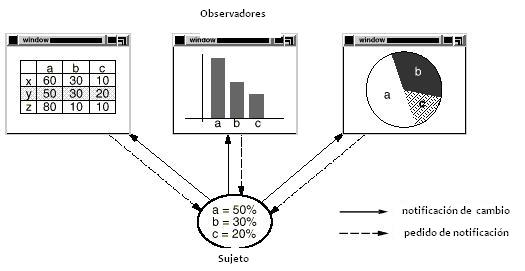
\includegraphics[scale=0.8]{images/pattern_observer.jpg}
				\caption{Patr\'on Observer.} \label{pattern_observer}
			\end{figure}

	    	\subsubsection{Aplicabilidad}
	    	Se usa el patr\'on $Observer$ cuando: 
		    \begin{itemize}
    			\item Una abstracci\'on tiene dos aspectos, uno dependiente del otro. Encapsular estos aspectos en objetos por separado le permite variarlo y 
    			reutilizarlos de manera independiente.
			    \item Un cambio de un objeto requiere cambiar a los dem\'as, y no se sabe cuantos objetos hay que cambiar.
				\item Un objeto debe ser capaz de notificar a otros objetos sin hacer suposiciones acerca de qu\'e son estos objetos. En otras palabras, no se 
				quiere que los objetos est\'en muy acoplados.
		    \end{itemize}


\bibliography{biblio}
\addcontentsline{toc}{chapter}{Bibliography}
\bibliographystyle{apalike}
\end{document}
